\documentclass[12pt,a4paper]{article}

%% Paquetes
\usepackage[margin=2.5cm]{geometry}
\usepackage[utf8]{inputenc}
\usepackage[T1]{fontenc}
\usepackage{graphicx}
\usepackage{booktabs}
\usepackage{amsmath}
\usepackage{hyperref}
\usepackage[labelfont=bf,font=small]{caption}
\usepackage{subcaption}
\usepackage{lineno}
\usepackage{authblk}
\usepackage{setspace}
\usepackage{xcolor}
\usepackage{enumitem}
\usepackage[expansion=false]{microtype}
\usepackage{natbib}

\hypersetup{
  colorlinks=true,
  linkcolor=blue!60!black,
  citecolor=blue!60!black,
  urlcolor=blue!60!black
}

\doublespacing
\linenumbers

%% Metadatos del artículo (versión auditada 2026-05-08)
\title{\textbf{Análisis de consenso multi-método para transcriptómica espacial \textit{in situ} dirigida: marco analítico con demostración piloto en adenocarcinoma pulmonar humano}}

\author[1]{Miguel \'{A}ngel D\'{i}az-Campos}
\author[1,$\dagger$]{Alfredo de Jes\'{u}s Rodr\'{i}guez G\'{o}mez}
\affil[1]{Instituto Nacional de Pediatr\'{i}a (INP), Ciudad de M\'{e}xico, M\'{e}xico}
\affil[$\dagger$]{Autor de correspondencia: \href{mailto:alfredo.rodriguez@iibiomedicas.unam.mx}{alfredo.rodriguez@iibiomedicas.unam.mx}}

\date{}

\begin{document}

\maketitle

\begin{abstract}
Las tecnologías de transcriptómica espacial permiten la caracterización simultánea de la expresión génica y la organización celular en tejidos intactos; sin embargo, no existe una metodología de consenso para integrar múltiples marcos analíticos en inferencias biológicas reproducibles. En este trabajo presentamos un pipeline de consenso multi-herramienta para transcriptómica espacial \textit{in situ} y lo aplicamos a un conjunto de datos público de Xenium de adenocarcinoma acinar invasivo pulmonar humano (268,034 células, 289 genes; una sección de tejido, un paciente). Para cada familia analítica --- anotación, detección de genes espacialmente variables, inferencia de dominios espaciales, comunicación célula--célula y trayectorias de pseudotime --- se aplica al menos dos herramientas computacionales independientes y solo se retienen los hallazgos concordantes entre métodos. El marco identifica 288 de 289 genes con autocorrelación espacial significativa a través de tres pruebas ortogonales, dos particiones de dominios espaciales (Banksy y Novae) con 35.4\% de coincidencia a nivel celular bajo un criterio estricto (el 64.6\% restante representa células de borde o estados de transición entre dominios), y 20 de 30 interacciones candidatas de comunicación célula--célula validadas tanto por puntuación ligando--receptor con corrección Benjamini--Hochberg como por inferencia espacial bayesiana con corrección Bonferroni. El eje dominante validado involucra a la sheddasa ADAM17 y a la oncomucina MUC1, con señal de co-localización en seis poblaciones emisoras independientes (mieloides y estromales) que convergen sobre células tumorales (valores $p$ de Spacia entre $4.97 \times 10^{-31}$ y $1.10 \times 10^{-71}$). Dentro del compartimento macrofágico, una sub-trayectoria inferida independientemente por pseudotime de difusión y Slingshot (Métodos) revela un continuo de estados de activación --- \emph{no} una polarización direccional M1$\to$M2, ya que tanto los marcadores canónicos M1 como M2 incrementan a lo largo del pseudotime inferido --- que acompaña a esta arquitectura de señalización. Estos resultados, derivados de una sola sección de tejido, establecen un marco analítico reproducible para transcriptómica espacial dirigida; la generalización biológica a través de subtipos y estadios de adenocarcinoma pulmonar requerirá validación en cohortes de pacientes.
\end{abstract}

\tableofcontents
\newpage

\section*{Introducción}
\label{sec:intro}
El desarrollo de plataformas de transcriptómica espacial \textit{in situ} ha transformado la biología tisular al permitir la medición simultánea de la expresión génica y el contexto espacial a resolución de célula única \citep{moses2022museum}. Entre estas tecnologías, la plataforma Xenium de 10x Genomics ofrece detección subcelular de transcritos en paneles de genes dirigidos de 100 a 5,000 genes, lo que la hace adecuada para el perfilado clínico de tejidos de forma rápida y rentable \citep{janesick2023high}. Sin embargo, la naturaleza dirigida de estos paneles --- típicamente de 289 a 480 genes --- plantea desafíos analíticos significativos: los métodos de reducción de dimensionalidad y agrupamiento desarrollados para datos de transcriptoma completo pueden rendir por debajo de lo esperado, la anotación de tipos celulares queda limitada por la disponibilidad de marcadores, y la detección de genes espacialmente variables debe operar sobre un universo génico preseleccionado.

Un desafío fundamental y subestimado en el análisis de transcriptómica espacial es la discordancia metodológica. Las herramientas computacionales independientes aplicadas al mismo conjunto de datos producen rutinariamente asignaciones de tipos celulares distintas, diferentes conjuntos de genes espacialmente variables y predicciones divergentes de comunicación célula--célula \citep{dimitrov2022comparison, efremova2020cellphonedb}. Sin una estrategia razonada para reconciliar estas discrepancias, resulta difícil distinguir señales biológicamente robustas de artefactos específicos de cada herramienta. Los enfoques de consenso --- que exigen confirmación independiente de al menos dos métodos ortogonales --- han sido defendidos en ómica de volumen y de célula única, pero no se han aplicado sistemáticamente a flujos de trabajo de transcriptómica espacial \citep{luecken2019current}.

El adenocarcinoma pulmonar representa un contexto biológico convincente para este tipo de marco analítico. El microambiente tumoral (TME) del adenocarcinoma pulmonar se caracteriza por una compleja comunicación intercelular entre células epiteliales malignas, poblaciones mieloides y subconjuntos del sistema inmune adaptativo, aunque la organización espacial de estas interacciones permanece incompletamente comprendida \citep{laughney2020regenerative, wu2021single}. En particular, los estados de polarización de los macrófagos y sus interacciones ligando--receptor con células tumorales han emergido como determinantes clave de la respuesta a inmunoterapia \citep{cassetta2020targeting}, pero la evidencia espacial directa de los ejes de señalización dominantes en tejido FFPE intacto ha sido limitada por la escasez de validaciones espaciales resueltas por tipo celular.

Aquí presentamos un pipeline modular y reproducible de consenso multi-herramienta para transcriptómica espacial \textit{in situ} dirigida y lo aplicamos a un conjunto de datos público de Xenium de adenocarcinoma acinar invasivo pulmonar humano (Estadio IB, 268,034 células, 289 genes; 10x Genomics CG000709). Para cada familia analítica --- anotación de tipos celulares, detección de genes espacialmente variables, inferencia de dominios espaciales, comunicación célula--célula y pseudotime --- empleamos al menos dos herramientas independientes y retenemos únicamente los hallazgos confirmados por ambas (Figura~\ref{fig:1}). Demostramos que esta estrategia de consenso reduce sustancialmente los falsos positivos preservando señales biológicamente coherentes. Nuestro hallazgo biológico clave es una arquitectura inmunosupresora dominada por células mieloides centrada en el eje ADAM17--MUC1, espacialmente validada en seis tipos celulares emisores tras corrección Bonferroni, con valores $p$ ajustados que alcanzan $10^{-71}$, en línea con un modelo no-checkpoint de inmunosupresión mediada por sheddasa en el TME del adenocarcinoma pulmonar.

\begin{figure}[htbp]
\centering
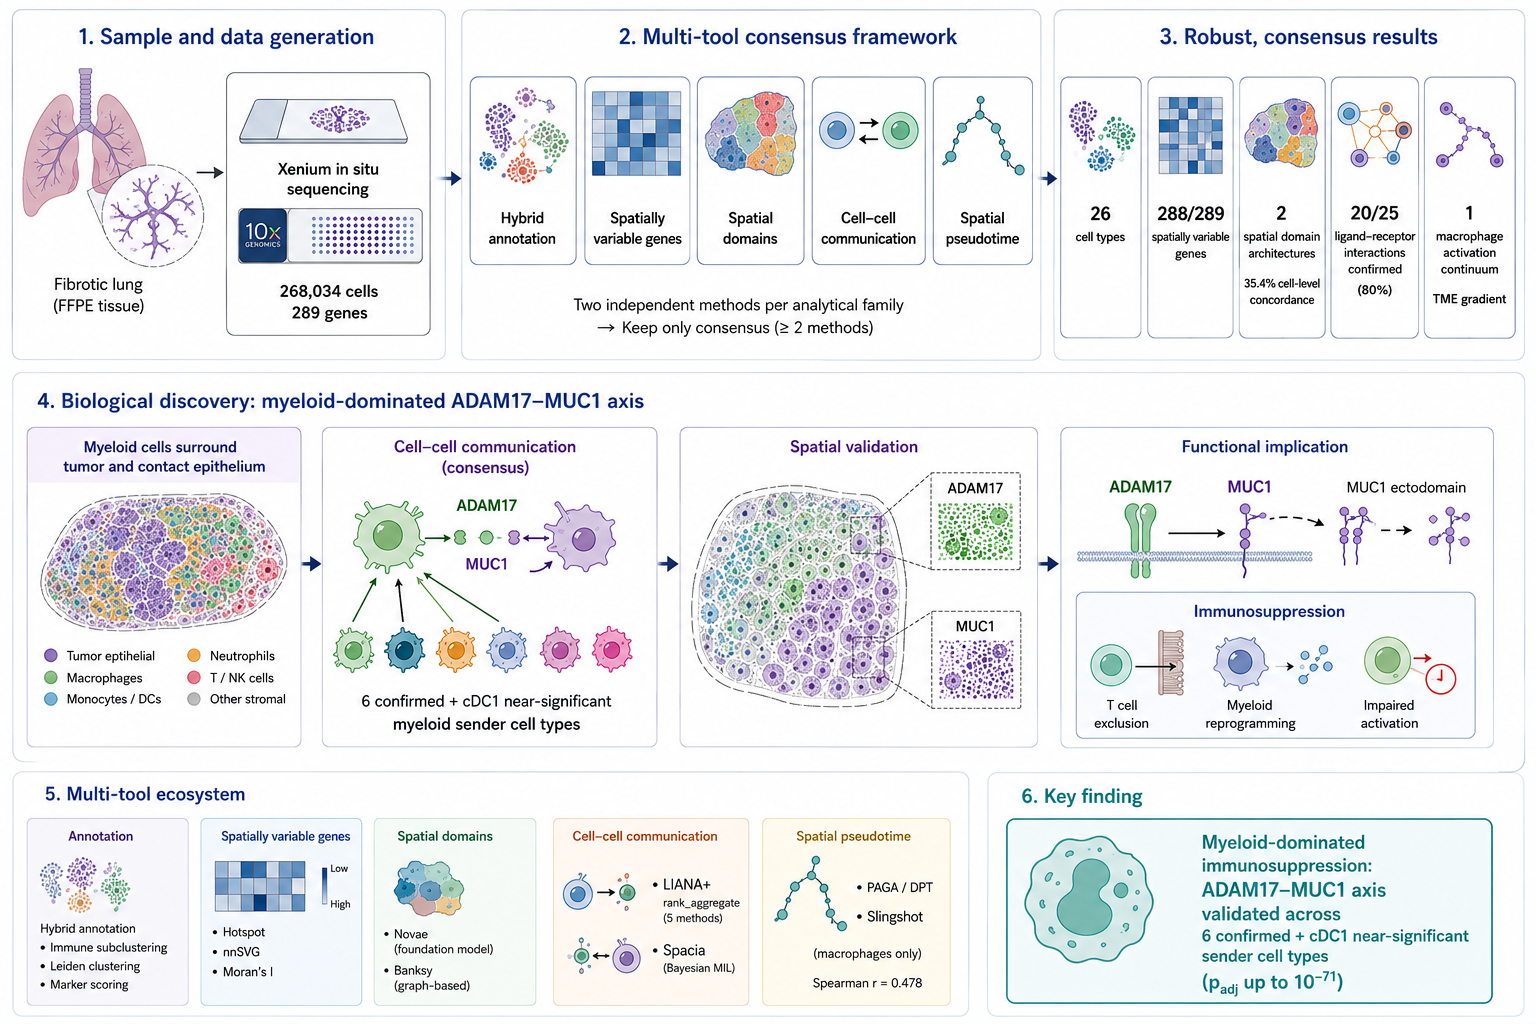
\includegraphics[width=\textwidth]{figures/Fig1A_Graphical_Abstract.png}
\caption{\textbf{Abstract gráfico del marco de consenso multi-herramienta y el hallazgo biológico principal.}
\textbf{(1)}~Generación de datos: tejido FFPE de adenocarcinoma pulmonar humano perfilado con la plataforma Xenium \textit{in situ} (panel de 289 genes, 268{,}034 células tras control de calidad).
\textbf{(2)}~Marco de consenso multi-herramienta: cada familia analítica (anotación híbrida, genes espacialmente variables, dominios espaciales, comunicación célula--célula, pseudotiempo espacial) atraviesa al menos dos métodos independientes y solo se retienen los hallazgos confirmados por $\geq 2$ métodos.
\textbf{(3)}~Resultados robustos de consenso: 26 tipos celulares; 288 de 289 genes espacialmente variables; dos arquitecturas complementarias de dominios espaciales con 35.4\% de coincidencia por célula bajo el filtro estricto de consenso; 20 de 25 interacciones de comunicación célula--célula completadas (80\%) confirmadas bajo la validación conjunta LIANA+/Spacia; un único continuo de activación macrofágica no direccional.
\textbf{(4)}~Hallazgo biológico: un eje de señalización ADAM17--MUC1 dominado por células mieloides. Las poblaciones mieloides rodean a las células tumorales y contactan al epitelio; el hub ADAM17--MUC1 se valida en seis tipos celulares emisores confirmados (más cDC1 a significancia per-test), espacialmente co-localizado con receptores tumorales, y consistente con exclusión de células T mediada por shedding y activación efectora reducida.
\textbf{(5)}~Ecosistema multi-herramienta usado por familia analítica.
\textbf{(6)}~Hallazgo clave: inmunosupresión dominada por mieloides vía el eje ADAM17--MUC1, validada en seis tipos celulares emisores confirmados ($p_{\text{adj}}$ hasta $10^{-71}$).}
\label{fig:1}
\end{figure}

\section*{Resultados}
\label{sec:results}

\subsection*{3.1 Arquitectura tisular y anotación de tipos celulares}
Aplicamos una estrategia de anotación híbrida de tres fuentes para asignar tipos celulares a las 268,034 células del conjunto post-QC (Figura Suplementaria~\ref{fig:s1}). La estrategia combinó subagrupamiento por linaje inmune basado en marcadores canónicos del panel, detección de comunidades Leiden a múltiples resoluciones, y un enfoque de puntuación con firmas génicas curadas para los compartimentos principales. Este enfoque de tres fuentes fue necesario porque ningún método individual capturaba simultáneamente poblaciones inmunes raras y subconjuntos estromales y epiteliales abundantes a la resolución requerida para los análisis posteriores.

La taxonomía final comprende 14 categorías celulares amplias, 26 subtipos granulares y 7 estados funcionales. Las categorías incluyen linajes epiteliales (alveolar tipo 1 y tipo 2, ciliadas y epitelio general), poblaciones estromales (endoteliales --- incluido el endotelio linfático ---, pericitos, fibroblastos), compartimentos inmunes (macrófagos en estados M1- y M2-like, monocitos clásicos e intermedios, subtipos de dendríticas: cDC1, cDC2 y plasmacitoides pDC, células T, NK, B, plasmáticas y plasmablastos), y poblaciones tumorales epiteliales activamente proliferantes y en reposo (Figura~\ref{fig:2}).

Para evaluar la estabilidad interna de la anotación, calculamos el adjusted Rand index (ARI) entre la asignación híbrida primaria y un re-corrido del subagrupamiento de linaje inmune utilizando solo esa fuente (sin las etapas de Leiden y de puntuación de firmas). El ARI resultante de 0.742 cuantifica la estabilidad interna a través de usos complementarios del panel y se utilizó para informar la confianza por agrupamiento; señalamos explícitamente que se trata de una métrica de consistencia interna y no de una validación independiente basada en una referencia externa, ya que las tres fuentes operan sobre el mismo panel de 289 genes y dependen parcialmente de una lógica de marcadores compartida. La validación basada en referencias contra un atlas público de scRNA-seq pulmonar no fue posible aquí porque el panel dirigido de 289 genes no contiene los marcadores requeridos por los métodos de mapeo a referencia preentrenados actuales (e.g., CellTypist Human\_Lung\_Atlas requiere $>$2,000 genes); intentamos CellTypist de cualquier forma y observamos colapso a 4--5 clases amplias (resultados no reportados), confirmando que el mapeo a referencia para paneles dirigidos queda actualmente fuera del régimen operativo de estas herramientas. El 4.8\% de células asignadas como Unassigned representa células con perfiles de marcador ambiguos, consistentes con estados de transición o dobletes no resolubles a 289 genes de resolución.

Espacialmente, los tipos celulares anotados muestran una fuerte compartimentalización tisular (Figura~\ref{fig:2}). Las células tumorales se concentran en estructuras glandulares, mientras que las células alveolares tipo 1 y tipo 2 ocupan el parénquima alveolar adyacente. Los macrófagos y dendríticas se distribuyen a lo largo del estroma y en la interfaz tumor--parénquima, consistente con su papel de células centinela en el TME. Esta arquitectura provee el sustrato celular para los análisis de comunicación y trayectoria descritos a continuación.

\begin{figure}[htbp]
\centering
\begin{subfigure}[b]{0.48\textwidth}
  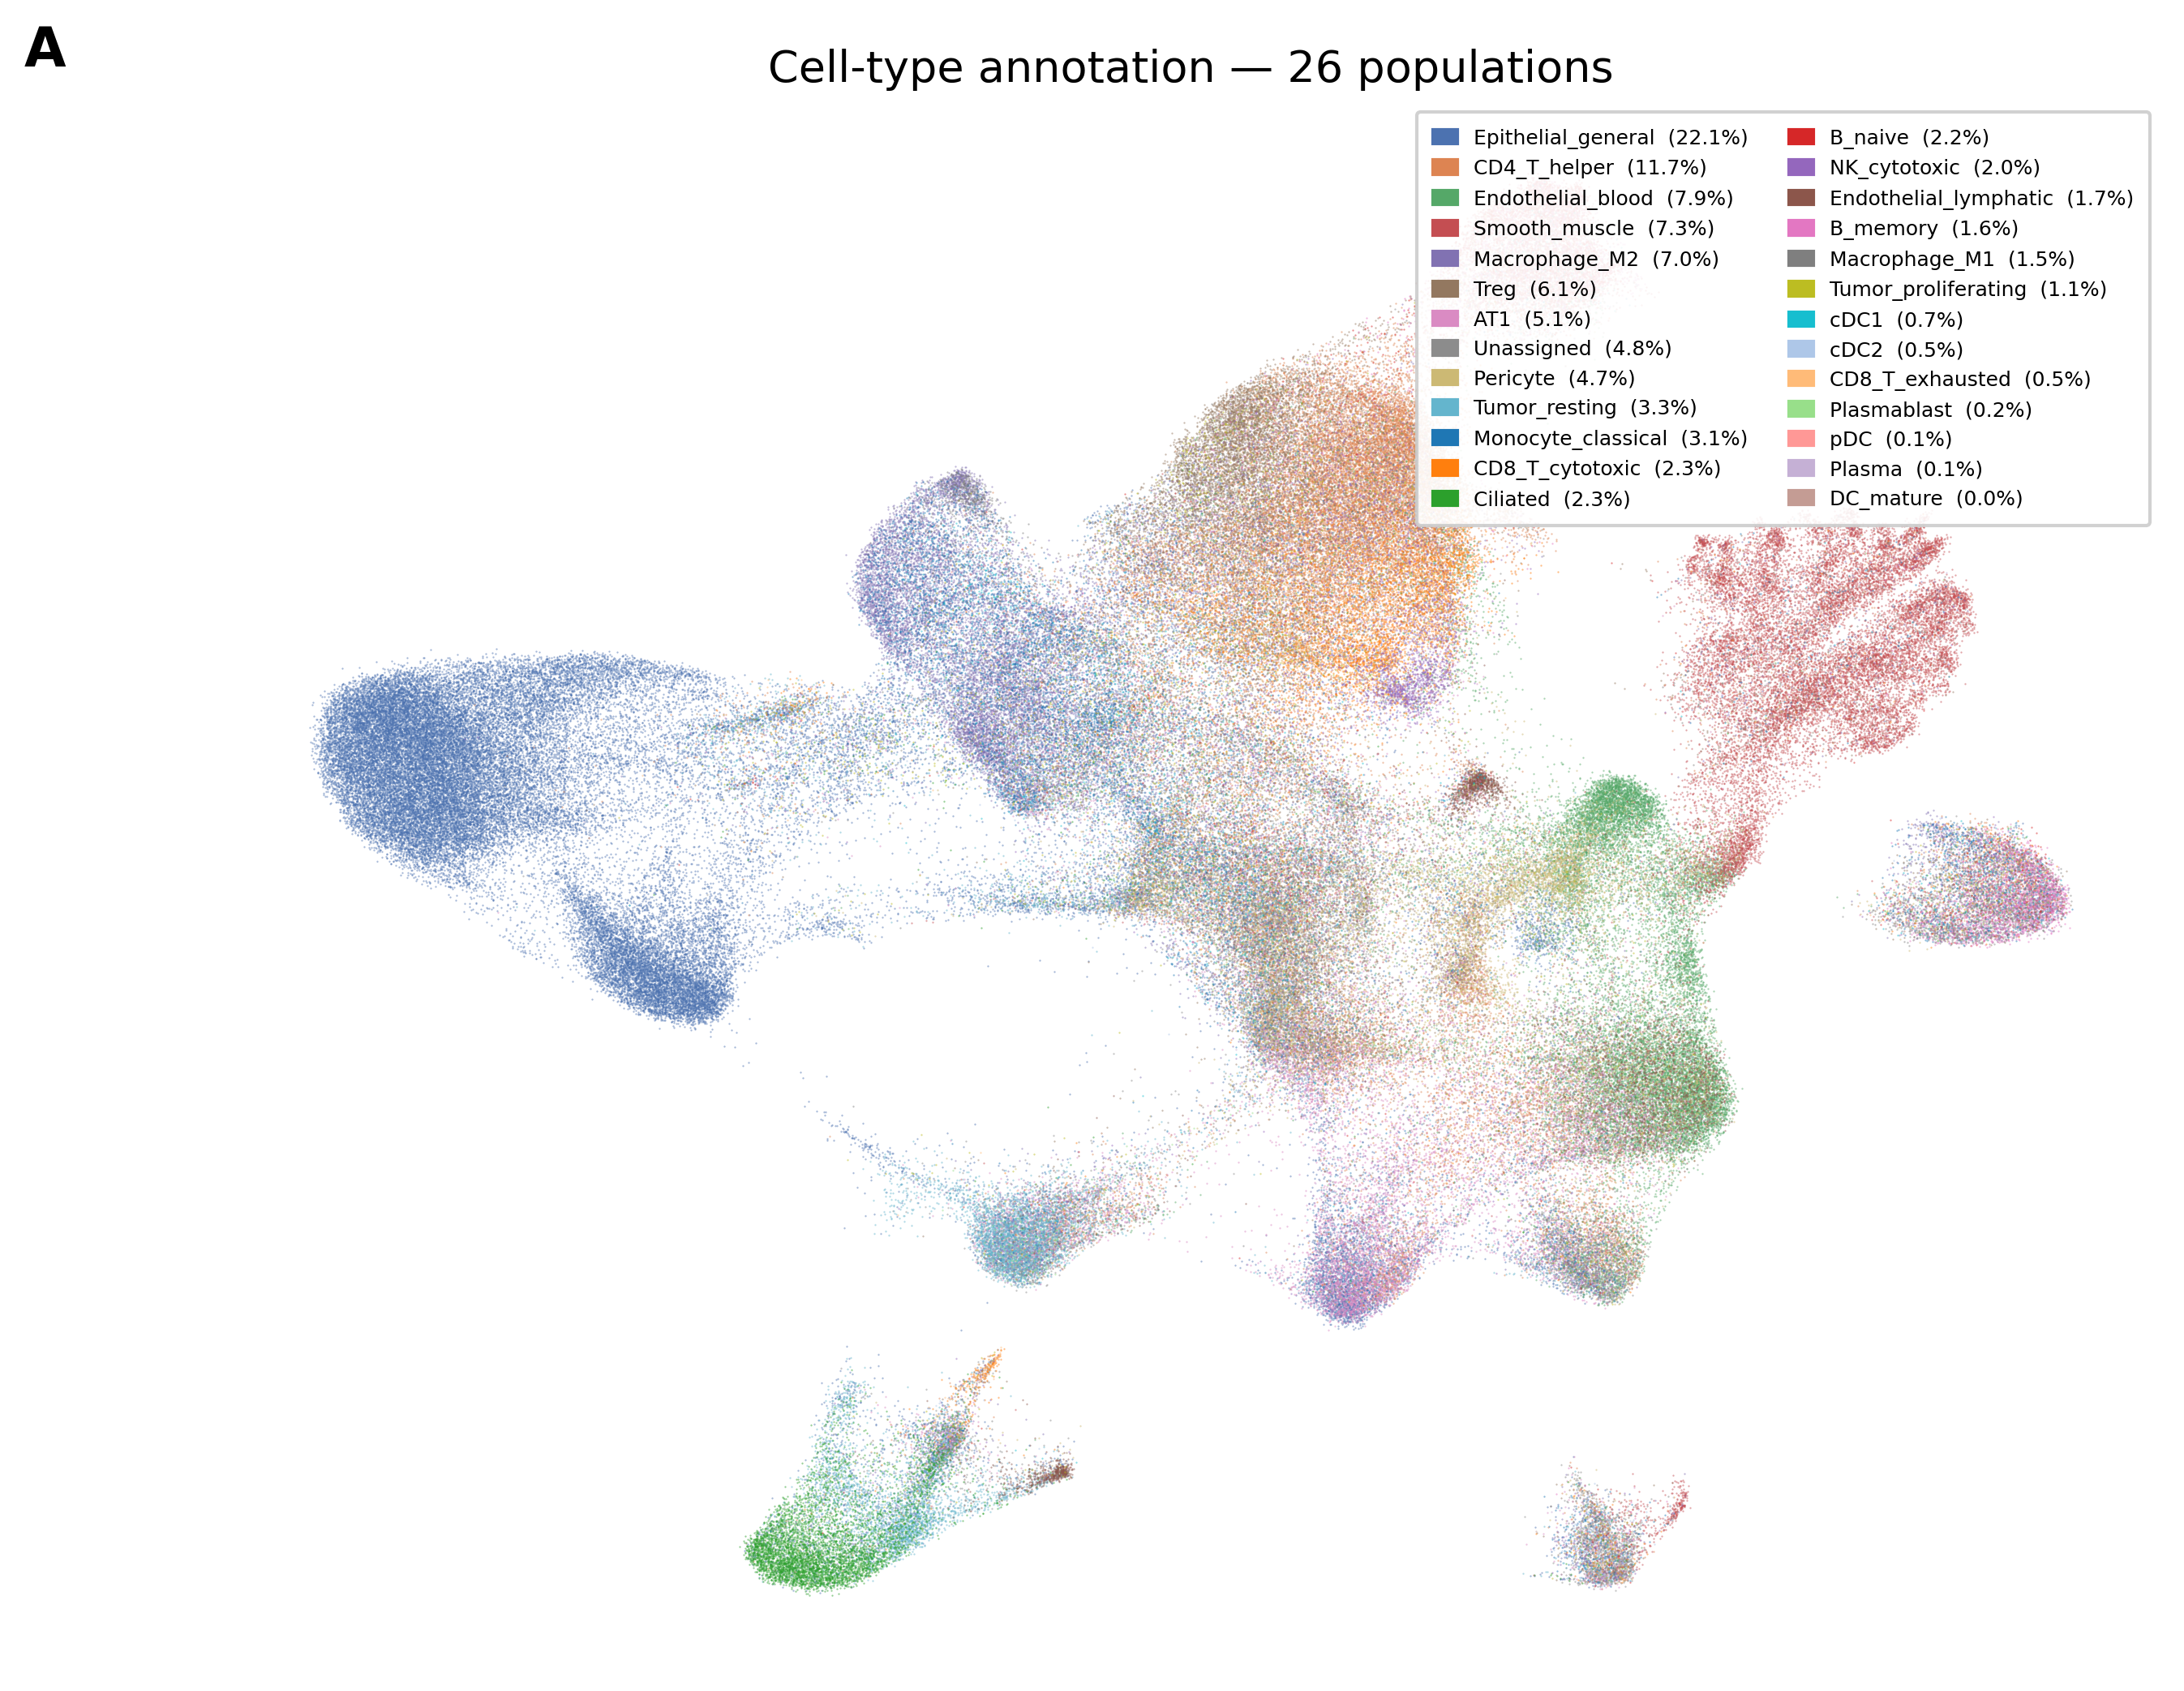
\includegraphics[width=\textwidth]{figures/Fig2A_umap_celltypes.png}
  \caption{}
  \label{fig:2a}
\end{subfigure}
\hfill
\begin{subfigure}[b]{0.48\textwidth}
  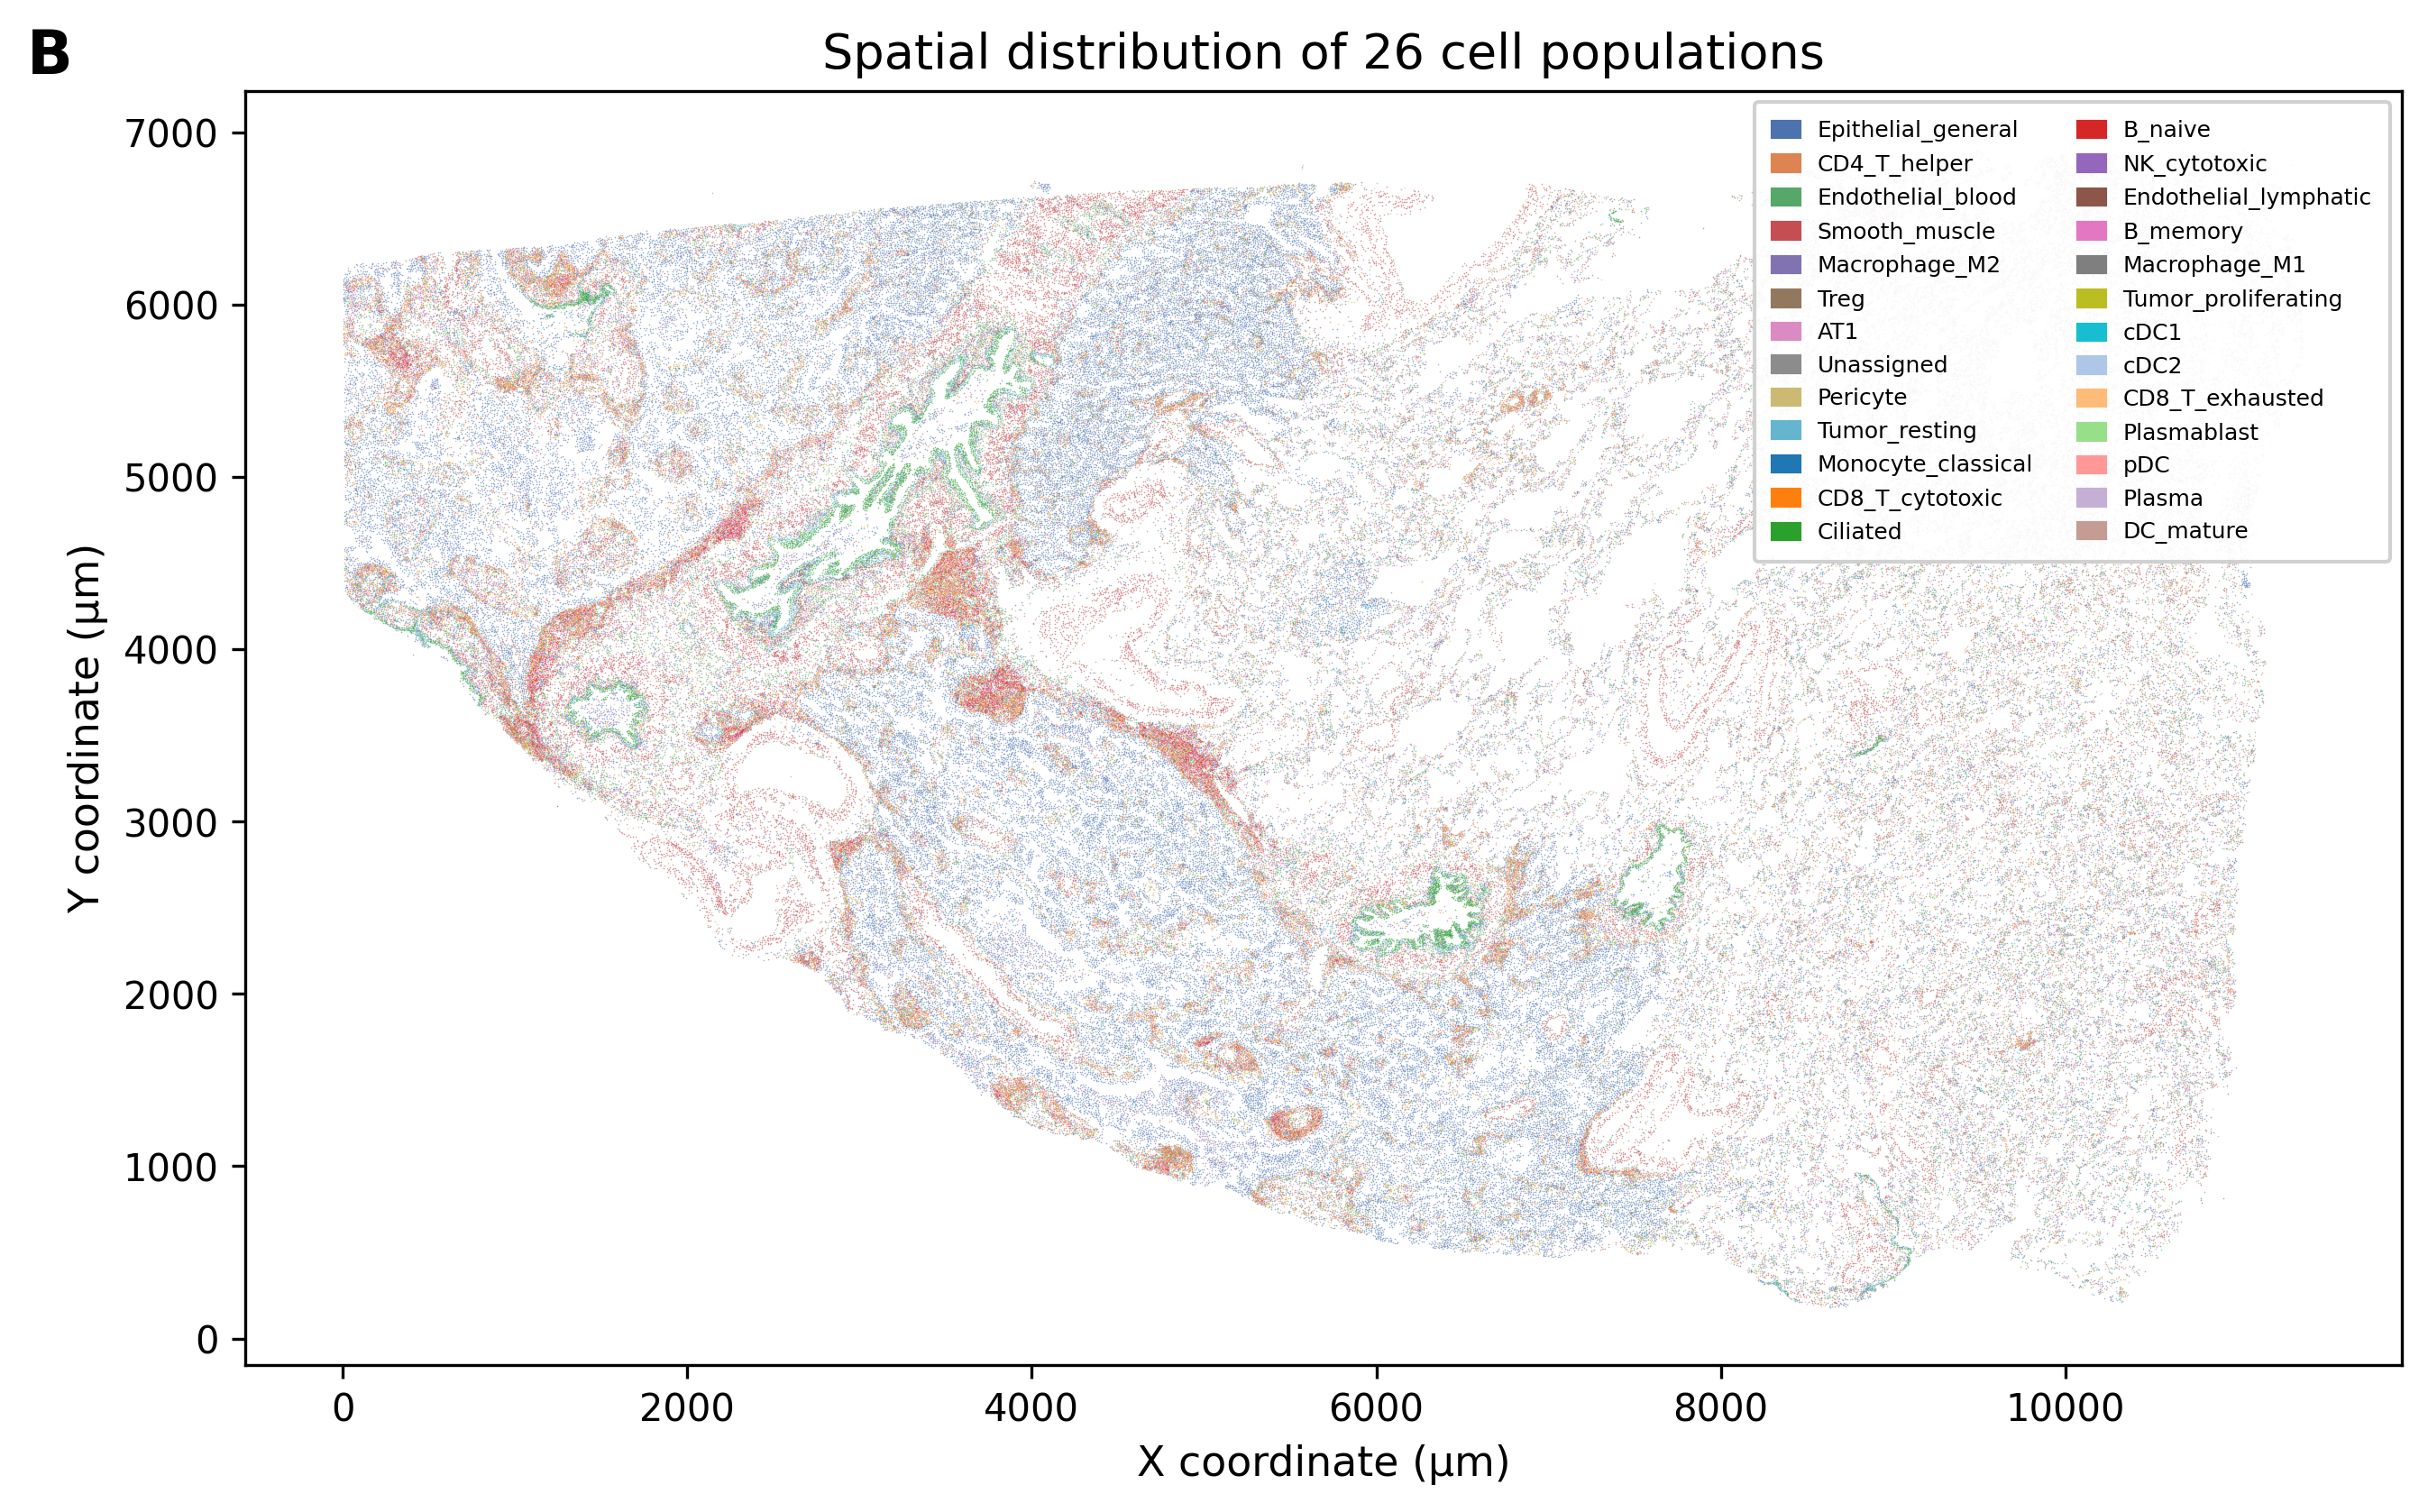
\includegraphics[width=\textwidth]{figures/Fig2B_spatial_celltypes.png}
  \caption{}
  \label{fig:2b}
\end{subfigure}
\begin{subfigure}[b]{0.48\textwidth}
  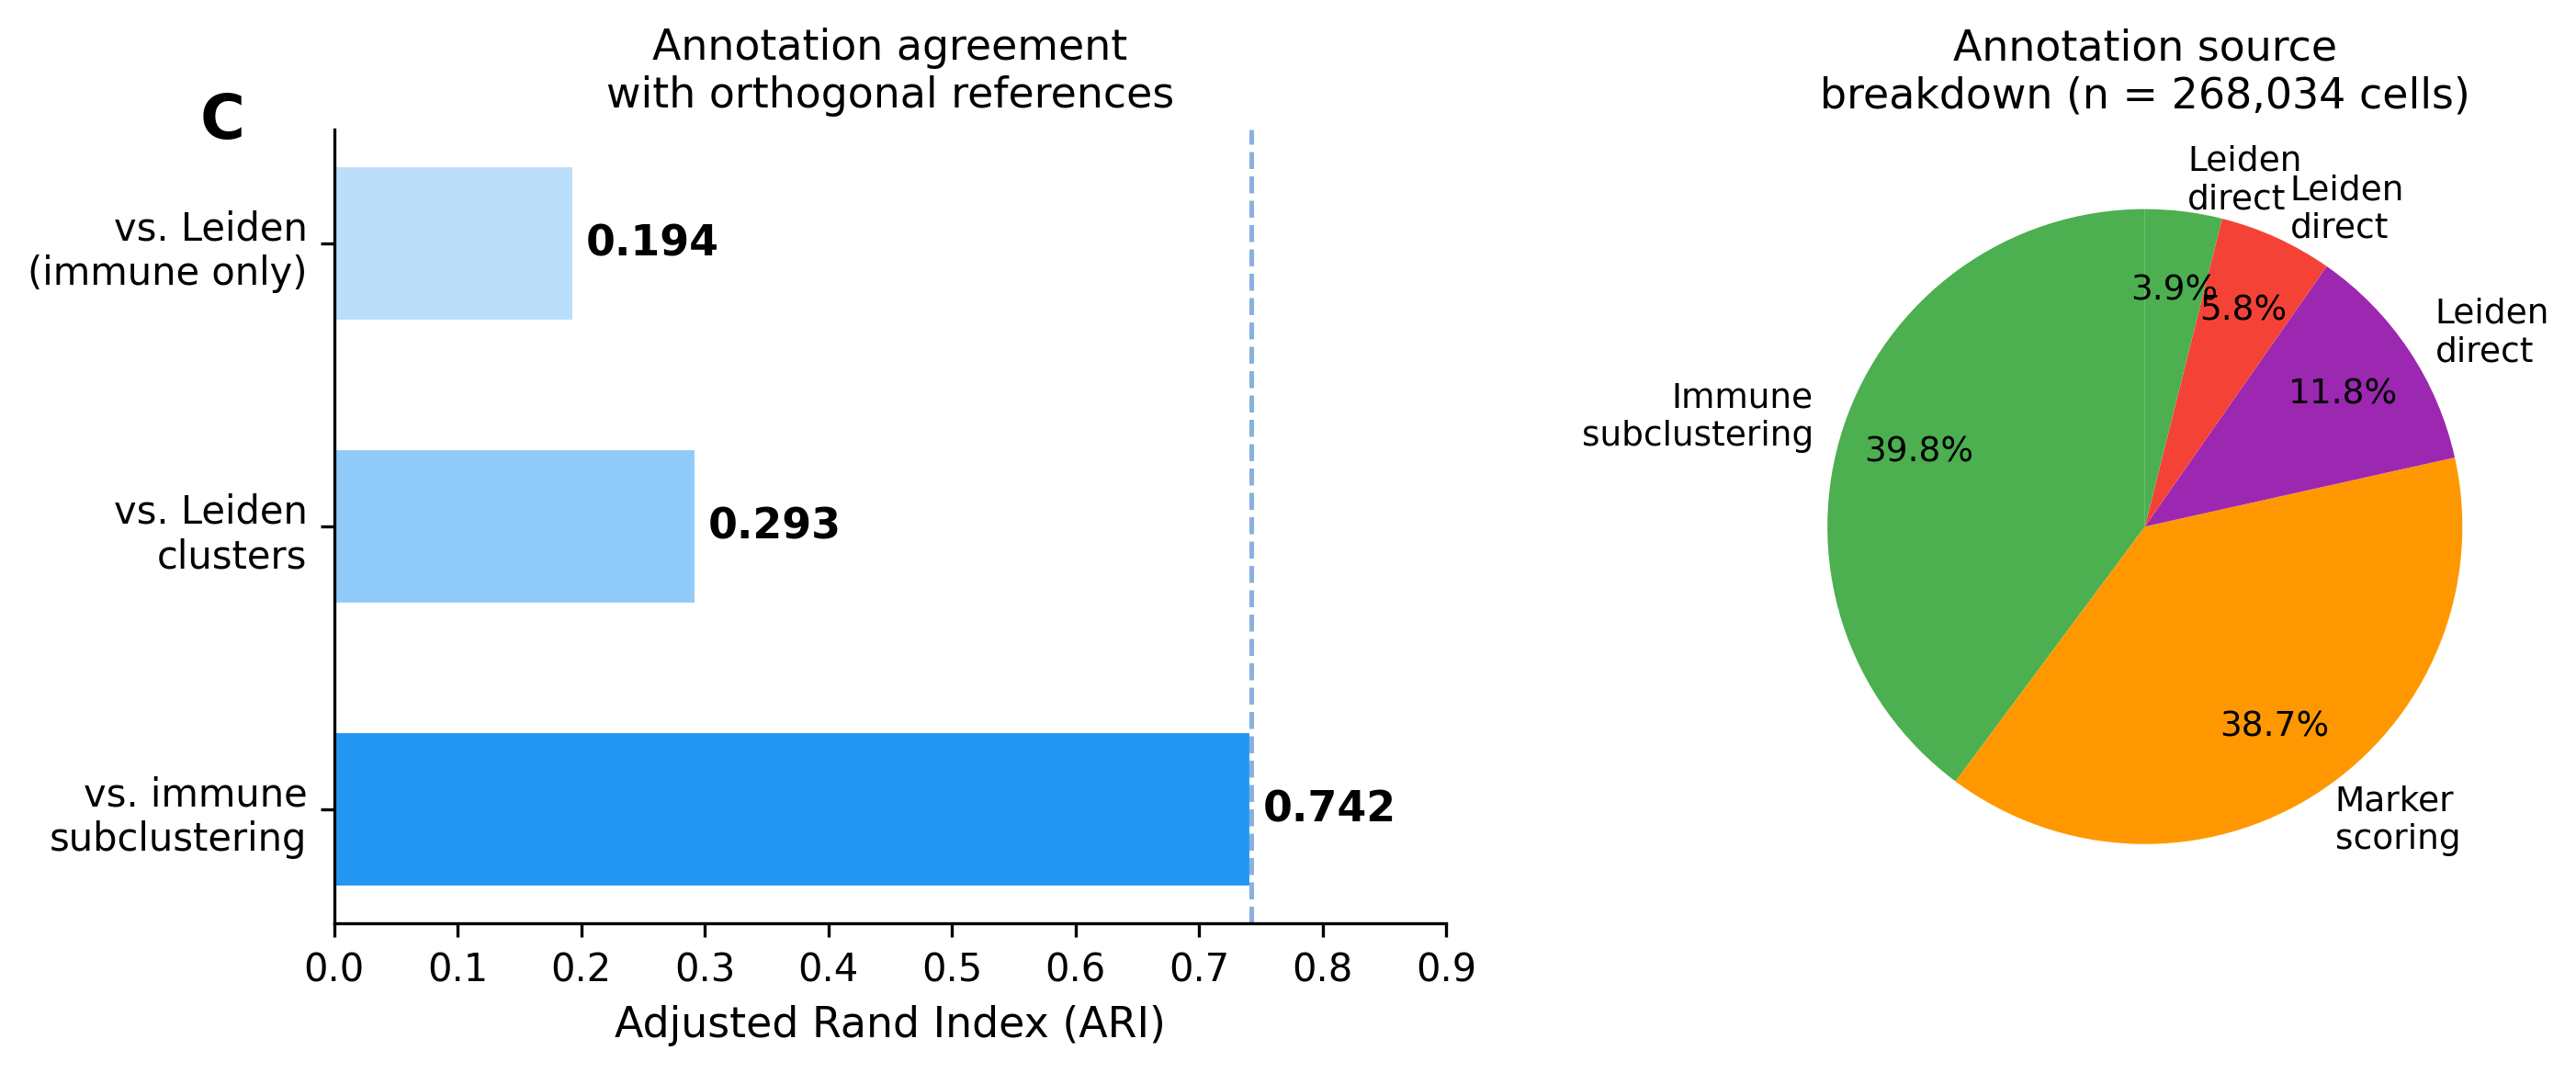
\includegraphics[width=\textwidth]{figures/Fig2C_annotation_validation.png}
  \caption{}
  \label{fig:2c}
\end{subfigure}
\caption{\textbf{Panorama de tipos celulares del microambiente tumoral del adenocarcinoma pulmonar.}
\textbf{(A)} UMAP de 268,034 células coloreadas por anotación granular (26 categorías).
\textbf{(B)} Distribución espacial de los tipos celulares anotados a través de la sección. Cada punto representa una célula; los colores corresponden al panel A.
\textbf{(C)} Comparación ARI entre la anotación híbrida primaria y el subagrupamiento inmune independiente (ARI = 0.742), reportado como métrica de estabilidad interna.}
\label{fig:2}
\end{figure}

\subsection*{3.2 Consenso de genes espacialmente variables}
Para identificar genes con patrones de expresión espacial no aleatorios, aplicamos tres métodos independientes de autocorrelación espacial al conjunto post-QC: Hotspot \citep{detomaso2021hotspot}, nnSVG \citep{weber2023nnsvg} y Moran's~I calculada vía Squidpy \citep{palla2022squidpy}. Cada método utiliza un marco estadístico distinto --- Hotspot emplea una prueba de autocorrelación local basada en vecindarios celulares; nnSVG ajusta procesos gaussianos no paramétricos teniendo en cuenta el tamaño de librería; Moran's~I cuantifica la autocorrelación espacial global mediante un grafo de adyacencia. Un gen se declaró SVG de consenso si alcanzó significancia estadística (FDR $<$0.05 o umbral equivalente) en al menos dos de los tres métodos.

De los 289 genes del panel Xenium, 288 (99.7\%) fueron identificados como SVGs de consenso, con un solo gen no alcanzando significancia en dos o más métodos. Esta estructura espacial casi universal es consistente con la naturaleza dirigida del panel Xenium, diseñado para incluir genes funcionalmente relevantes con patrones de expresión tejido-específicos conocidos \citep{janesick2023high}. La alta concordancia entre métodos valida la señal biológica más que reflejar falta de poder discriminativo: los tres métodos mostraron tasas de coincidencia por pares de 97--99\%, y el único gen discordante se caracterizó por baja expresión global (menos de 200 transcritos en todas las células). Reconocemos como caveat que esta tasa de 99.7\% de SVG-consenso refleja en parte el sesgo de selección del panel hacia genes con expresión espacial conocida; un análisis equivalente sobre un panel control no preseleccionado por especificidad espacial sería necesario para calibrar el poder discriminativo del marco (Discusión).

El agrupamiento de los 288 SVGs de consenso por patrón de expresión reveló módulos de coexpresión espacial correspondientes a los compartimentos tisulares principales: un módulo epitelial tumoral dominado por genes de proliferación y metabolismo, un módulo inmune enriquecido en marcadores de activación mieloide, y un módulo estromal asociado con remodelación de matriz extracelular. Estos módulos informaron el análisis de dominios espaciales descrito en la siguiente sección.

\subsection*{3.3 Inferencia de dominios espaciales}
Inferimos dominios tisulares espaciales mediante dos enfoques ortogonales. Novae \citep{schaar2025novae} es un foundation model preentrenado sobre atlas de célula única a gran escala; genera embeddings latentes de 64 dimensiones por célula que integran expresión y vecindario celular local, y los agrupa en dominios espaciales sin requerir un número de clusters definido por el usuario. Banksy \citep{zhao2023banksy} es un método basado en grafo que aumenta el perfil de expresión de cada célula con el perfil promediado de sus $k$ vecinos espaciales más cercanos ($\lambda = 0.2$, $k_{\text{geom}} = 6$), y luego aplica detección de comunidades Leiden para identificar agrupamientos espacialmente coherentes.

Banksy y Novae produjeron particiones de granularidad distinta, reflejando sus filosofías de diseño: Banksy produjo 14 dominios finos (B1--B14) sobre un grafo Leiden, mientras que el embedding del foundation model de Novae se agrupó en 10 dominios más amplios (D971--D1013) correspondientes a los compartimentos tisulares mayores. Las dos particiones no son por tanto correspondencia 1:1, y reportamos su relación como matriz de confusión en lugar de biyección por dominio (Figura Suplementaria~S2). Globalmente, el adjusted Rand index entre las dos particiones es ARI~$=0.15$ y la información mutua normalizada es NMI~$=0.31$, indicando desacuerdo sustancial a nivel de partición: los dos métodos no agrupan redundantemente la misma arquitectura sino que capturan escalas complementarias --- compartimentos amplios (Novae) frente a bordes finos (Banksy). Algunos dominios de Banksy mapean limpiamente a un único compartimento Novae (e.g., B5 $\to$ D998, 90\%; B8 $\to$ D1010, 76\%), y un criterio estricto de consenso por célula --- requiriendo que el dominio Banksy tenga un mejor-match Novae inequívoco y que la célula caiga en ese match --- retiene 35.4\% de las células (94,869 de 268,034) como asignaciones de alta confianza. El 64.6\% restante no es ruido aleatorio: se concentra en bordes de compartimento donde los dos métodos, por diseño, particionan de forma distinta. Enfatizamos que la tasa de 35.4\% cuantifica un filtro estricto post-hoc y no es equivalente a una alta concordancia de partición; el estadístico honesto de concordancia a nivel de partición es el ARI de 0.15. Los análisis posteriores que requieren todas las células (CCC y pseudotime) usaron el dataset completo anotado en lugar del subconjunto de consenso.

La arquitectura de dominios espaciales revela un núcleo tumoral claro rodeado de un anillo mieloide inmunosupresor: los dominios consenso cercanos al margen tumoral están enriquecidos en macrófagos M2-like y monocitos, mientras que los dominios internos tumorales están dominados por poblaciones tumorales epiteliales en reposo y proliferantes. Este motivo organizacional --- células mieloides posicionadas en la interfaz tumor--parénquima --- es consistente con exclusión inmune mediada por mieloides y establece el contexto físico para el análisis de comunicación ligando--receptor.

\begin{figure}[htbp]
\centering
\begin{subfigure}[b]{0.32\textwidth}
  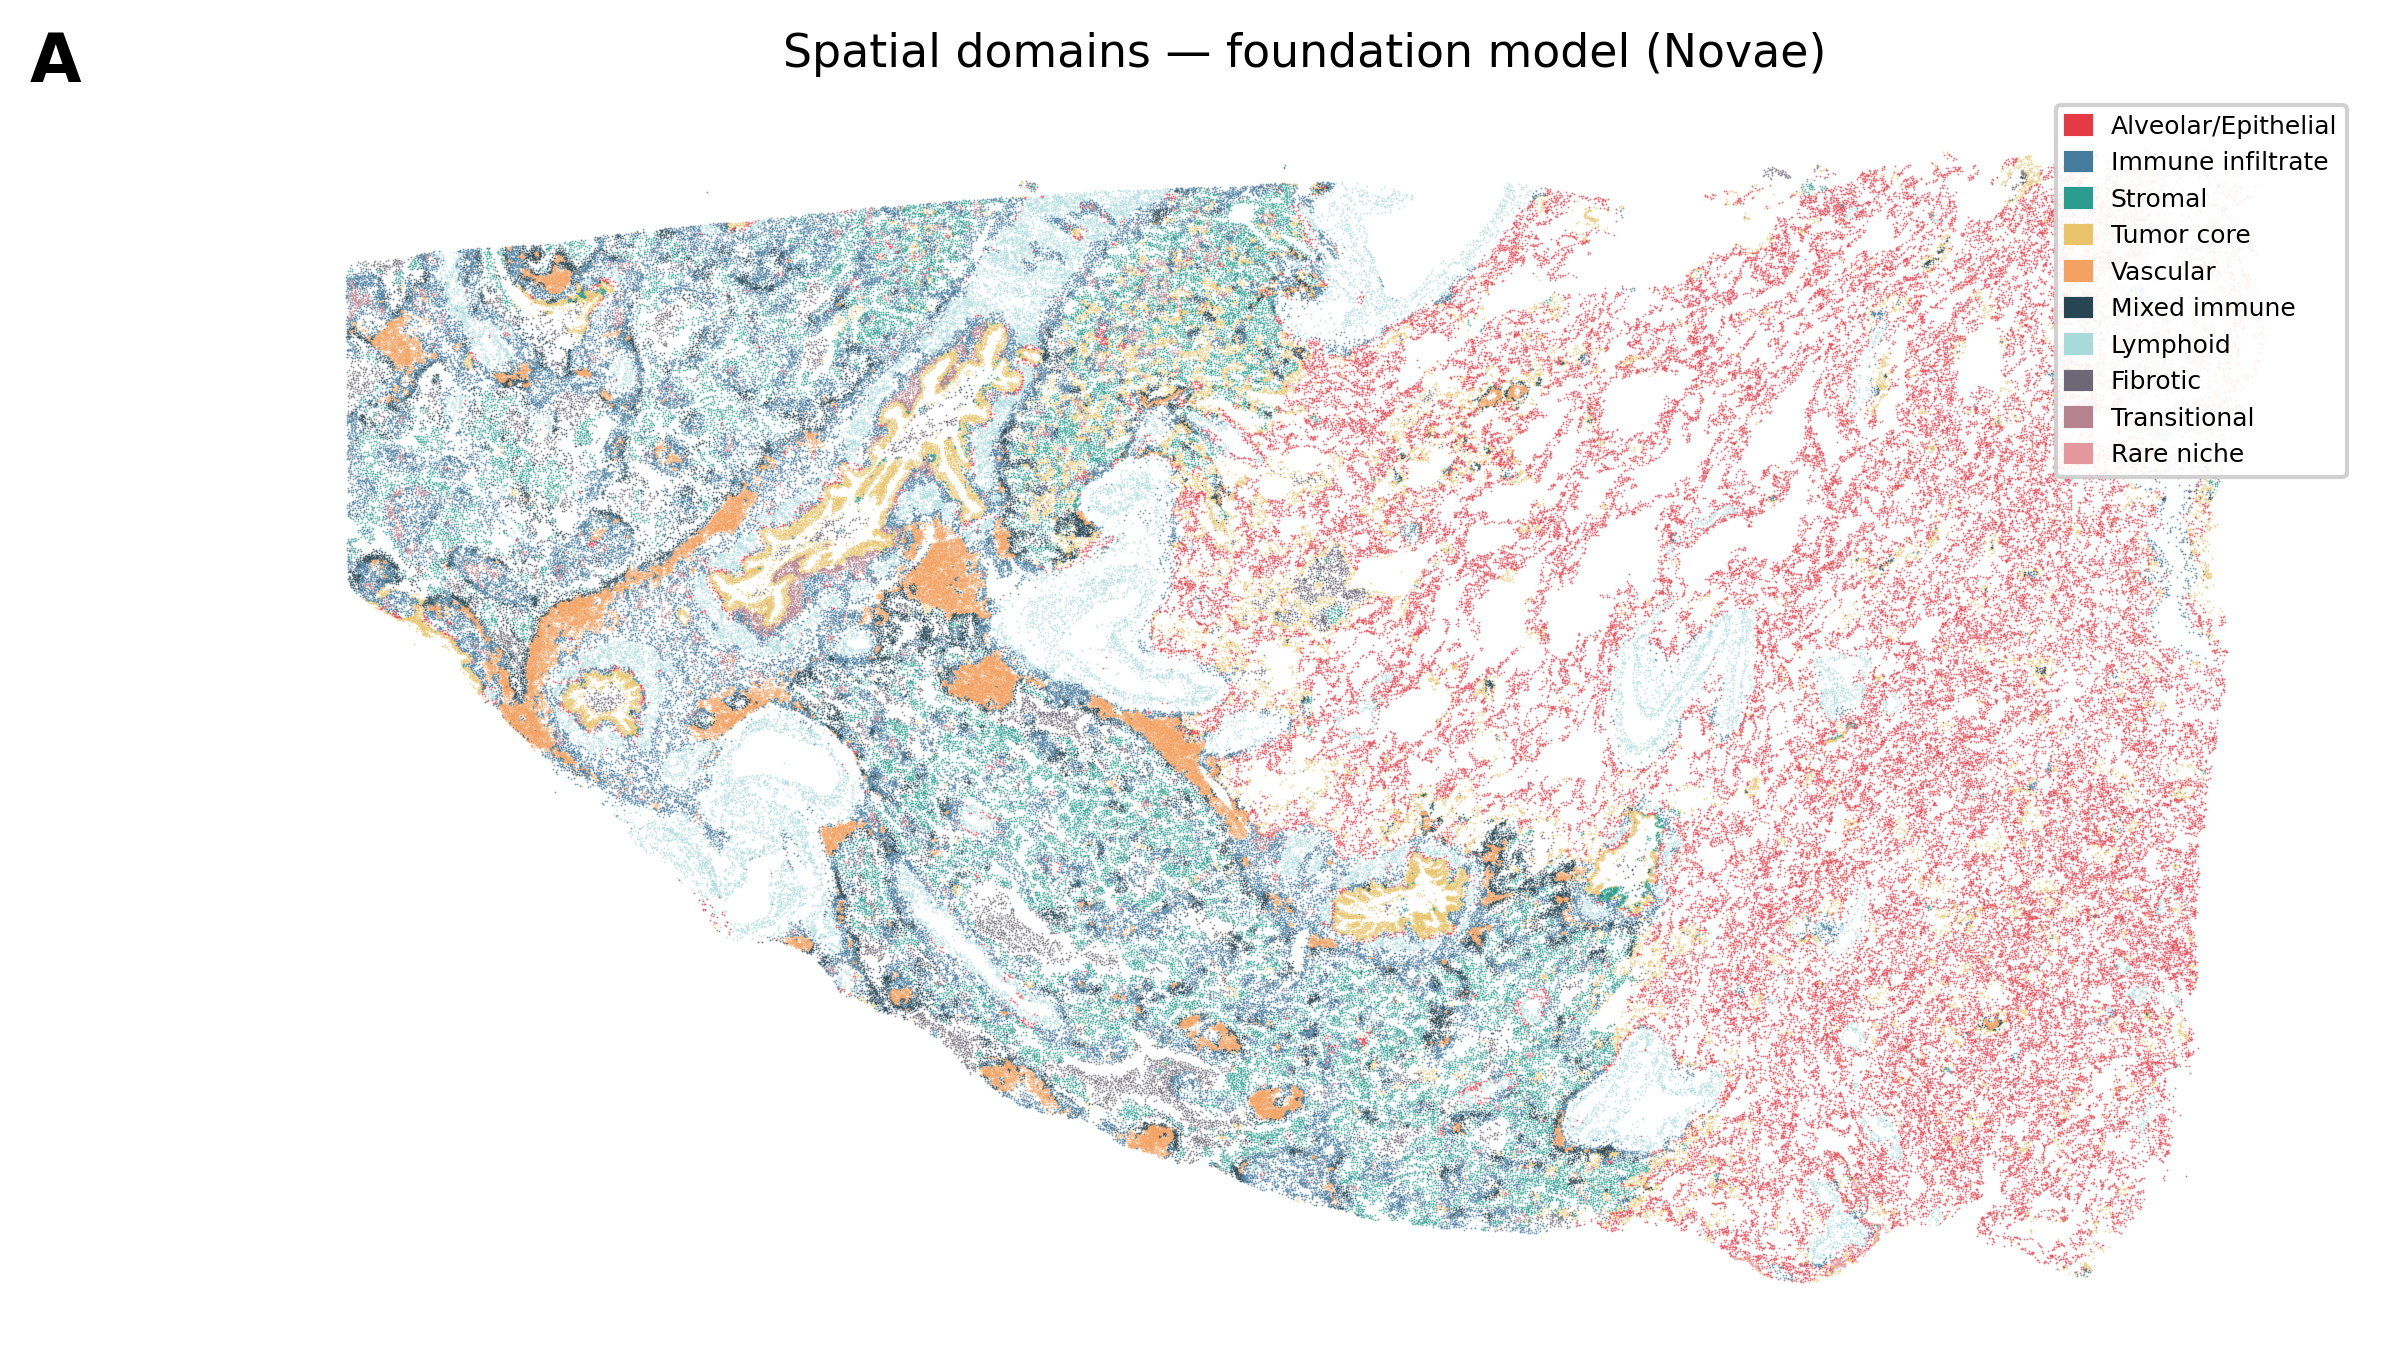
\includegraphics[width=\textwidth]{figures/Fig3A_novae_domains.png}
  \caption{Dominios Novae}
  \label{fig:3a}
\end{subfigure}
\hfill
\begin{subfigure}[b]{0.32\textwidth}
  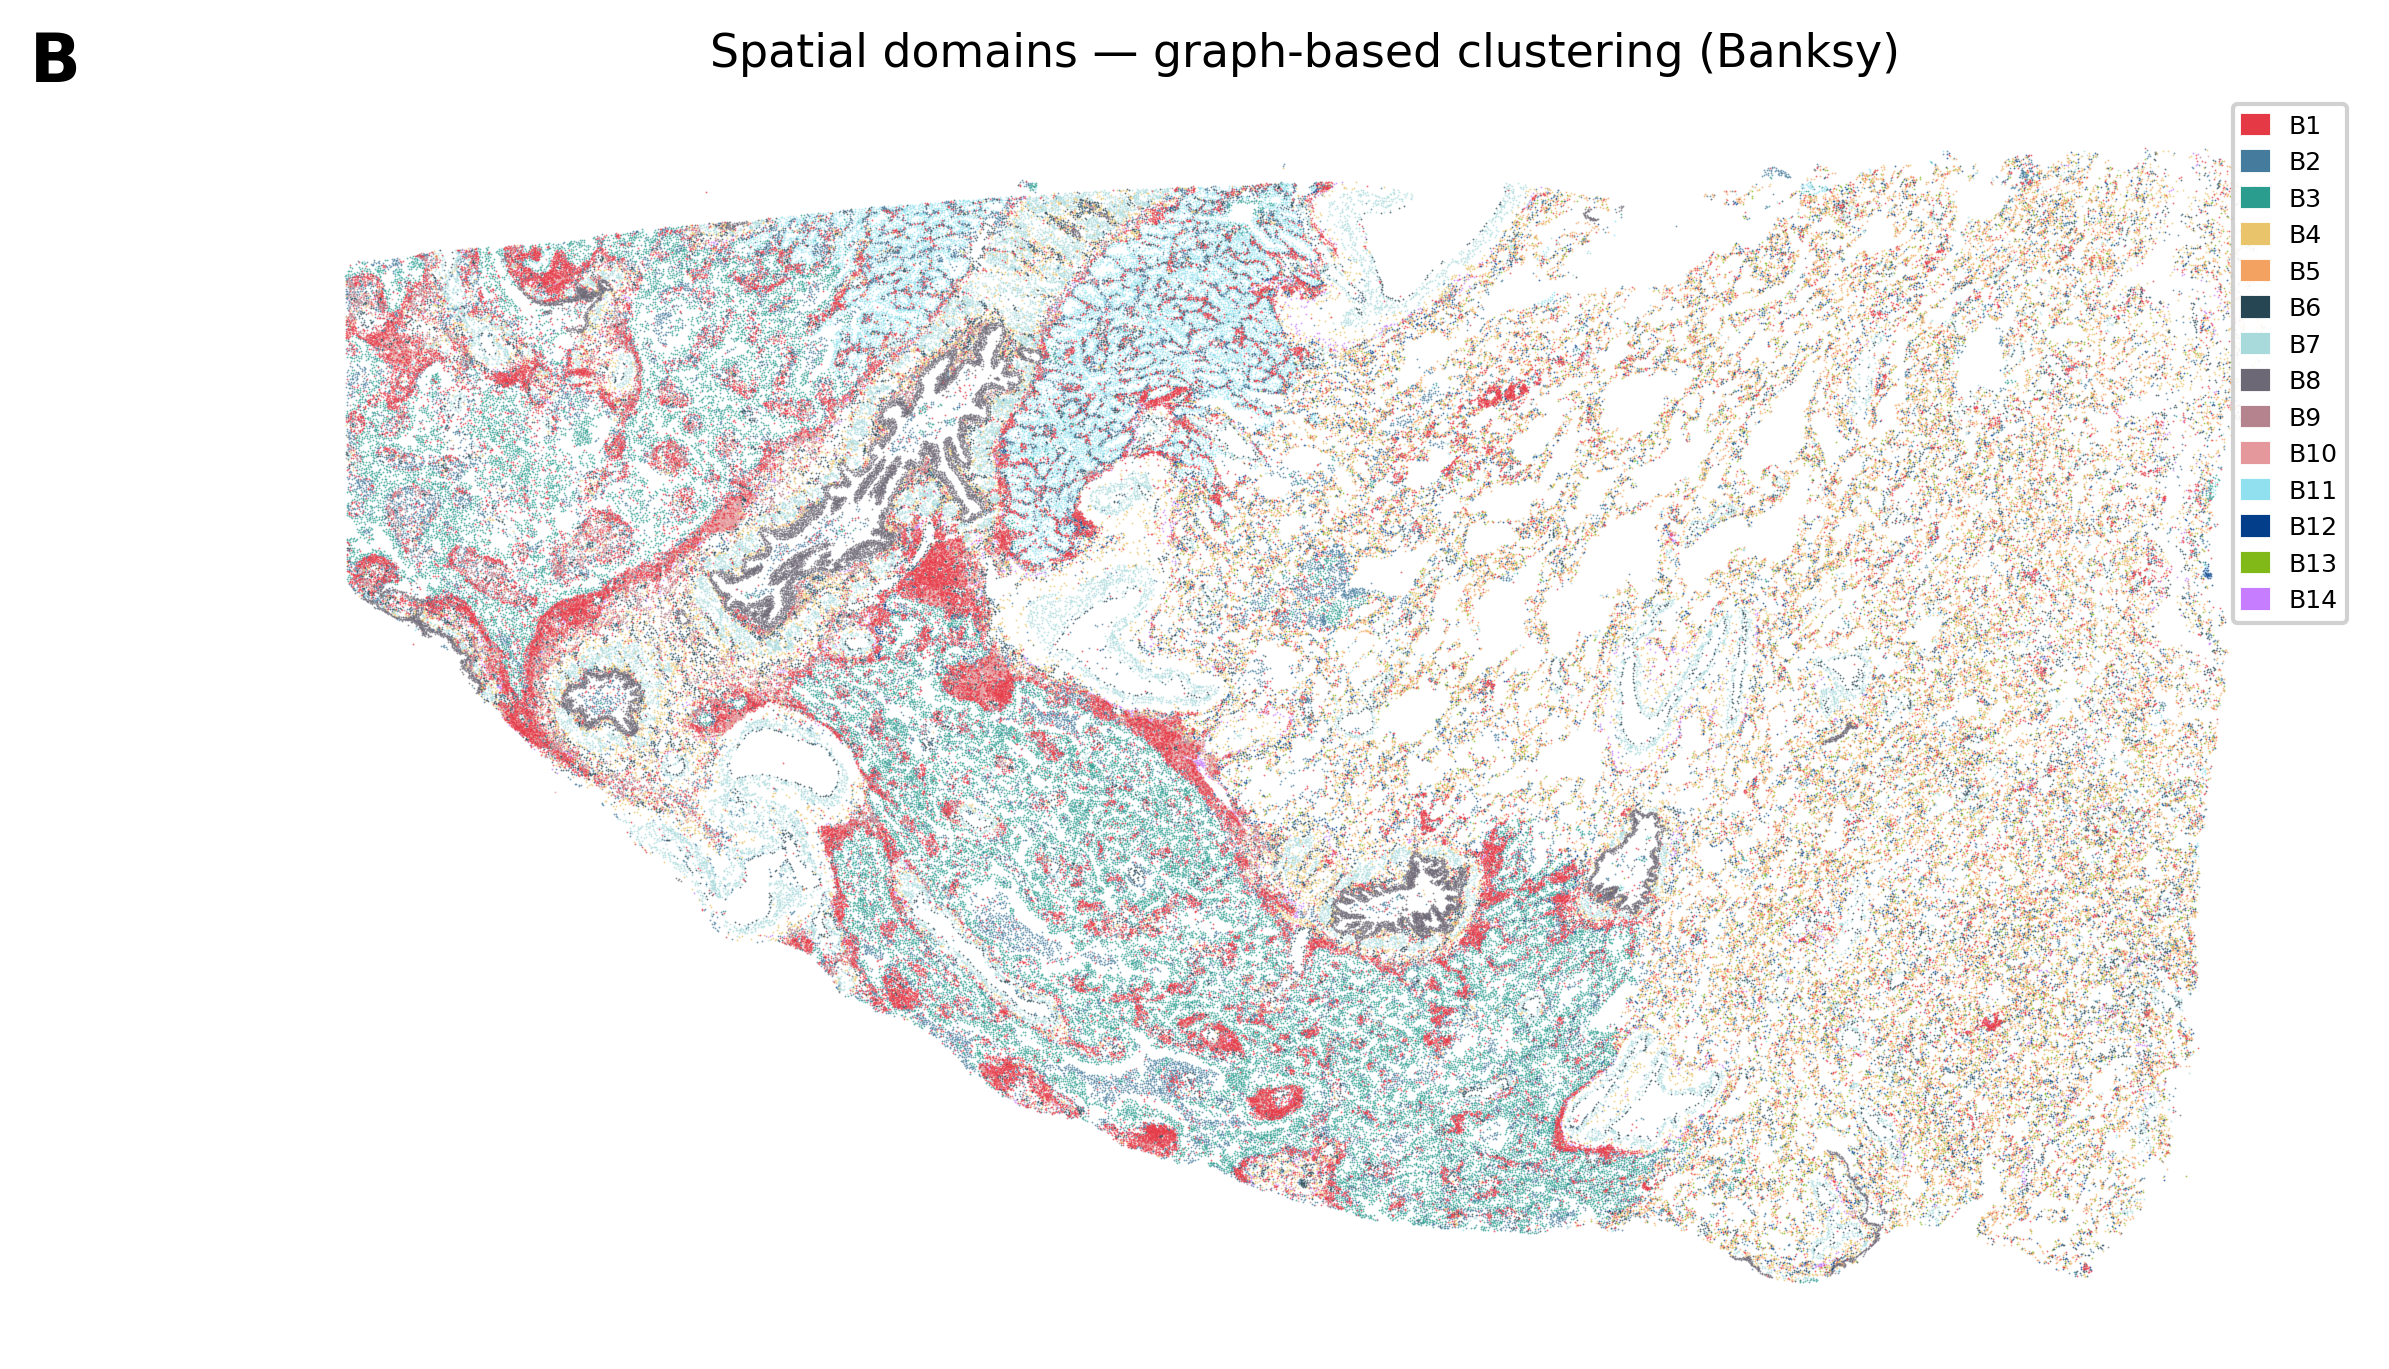
\includegraphics[width=\textwidth]{figures/Fig3B_banksy_domains.png}
  \caption{Dominios Banksy}
  \label{fig:3b}
\end{subfigure}
\hfill
\begin{subfigure}[b]{0.32\textwidth}
  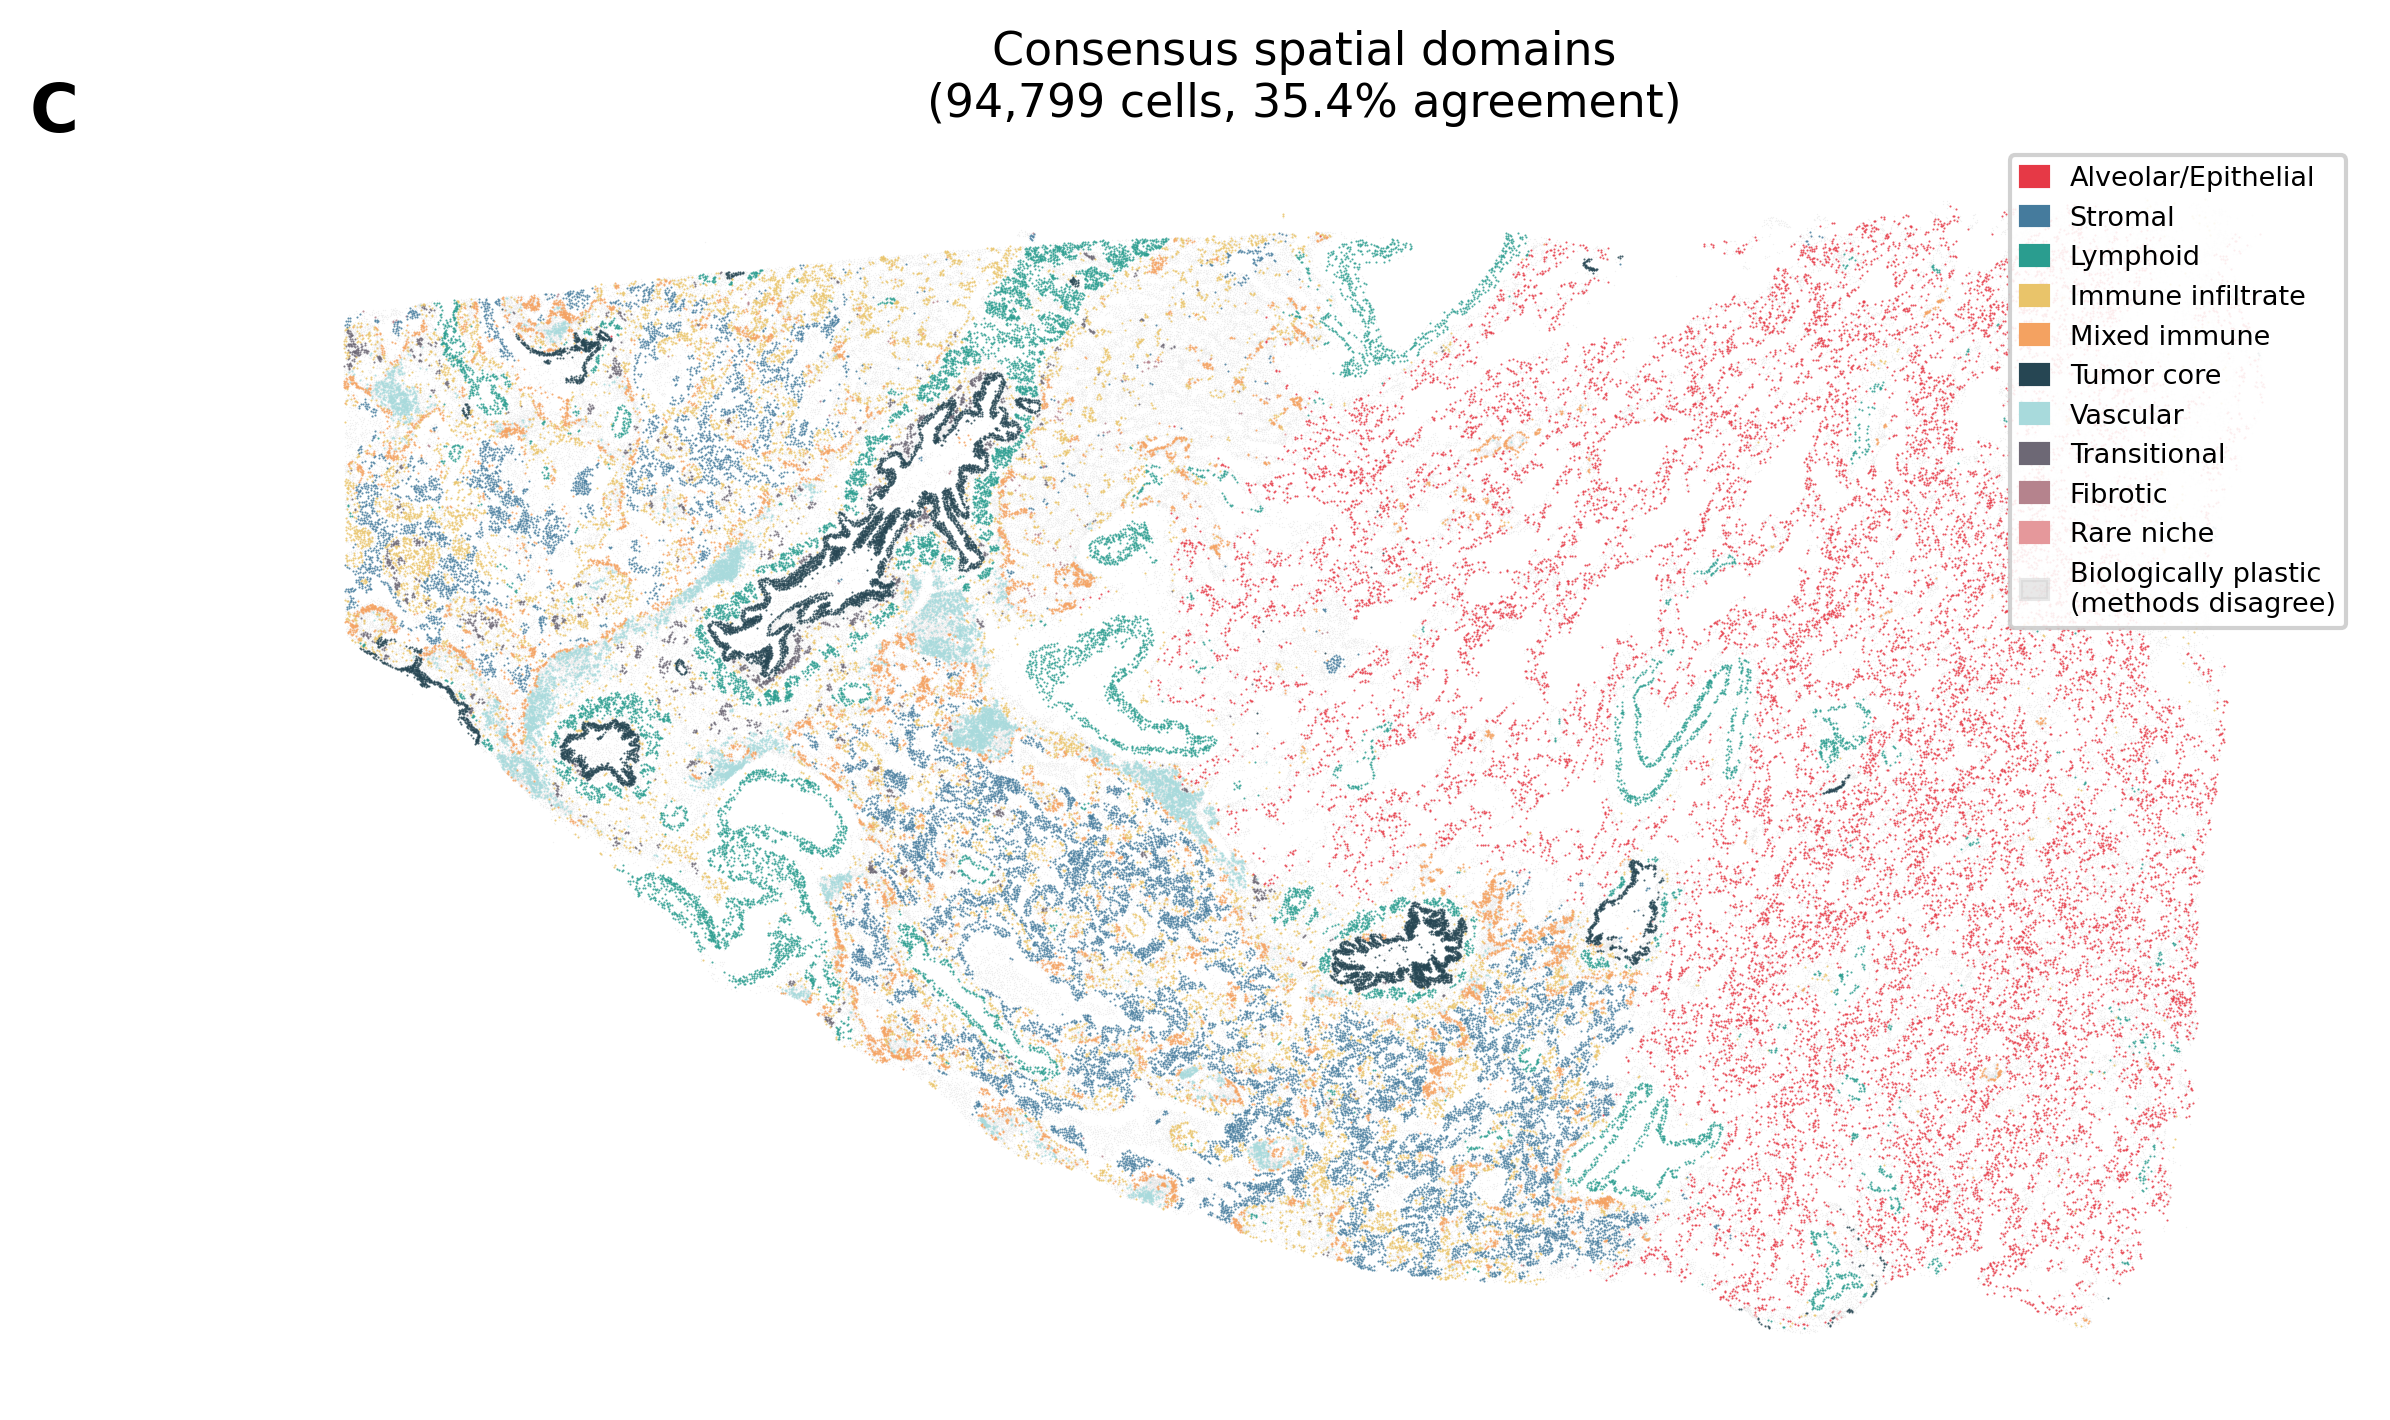
\includegraphics[width=\textwidth]{figures/Fig3C_consensus_domains.png}
  \caption{Consenso}
  \label{fig:3c}
\end{subfigure}
\caption{\textbf{Inferencia de dominios espaciales por dos métodos independientes.}
\textbf{(A)} Dominios Novae del foundation model (10 dominios, etiquetados D971--D1013; embeddings de 64 dimensiones agrupados sin forzar un $K$ objetivo).
\textbf{(B)} Dominios basados en grafo de Banksy (14 dominios, B1--B14; $\lambda = 0.2$, $k_{\text{geom}} = 6$).
\textbf{(C)} Asignación estricta de consenso por célula, definida como las células cuyo dominio Banksy tiene un mejor-match Novae inequívoco ($\geq 50\%$ de las células del dominio Banksy residen en ese dominio Novae) y que están asignadas a ese match: 94,869 células (35.4\%) en color, células sin consenso en gris. La concordancia a nivel partición entre los dos métodos es ARI~$=0.15$, NMI~$=0.31$ (Figura Suplementaria~S2): los métodos capturan escalas complementarias en lugar de agrupar redundantemente la misma arquitectura.}
\label{fig:3}
\end{figure}

\subsection*{3.4 Hubs de comunicación célula--célula validados dualmente}
Analizamos la comunicación célula--célula (CCC) usando una estrategia de validación dual que requirió confirmación independiente en dos niveles computacionales: puntuación ligando--receptor y co-localización espacial. En la primera etapa aplicamos LIANA+ \citep{ramirez2024liana} con el método \texttt{rank\_aggregate}, que combina evidencia de cinco algoritmos independientes de puntuación CCC (CellChat \citep{jin2021inference}, CellPhoneDB \citep{efremova2020cellphonedb}, NATMI \citep{hou2020predicting}, Connectome y scSeqComm). Los análisis se ejecutaron con 1,000 permutaciones, un radio espacial de 200~$\mu$m, y ponderación bivariada de coseno para tener en cuenta la proximidad espacial. Esto generó 2,631 pares de interacción (emisor $\times$ receptor $\times$ ligando $\times$ receptor; auto-interacciones excluidas). Los $p$-valores del componente CellPhoneDB se ajustaron a través de los 2,631 tests usando el procedimiento Benjamini--Hochberg, generando 1,557 interacciones a BH-FDR $<$ 0.05.

En la segunda etapa, las 30 interacciones de mayor magnitud por LIANA+ se sometieron a Spacia \citep{zhu2024spacia}, un marco bayesiano de aprendizaje por instancias múltiples que evalúa independientemente si las células emisoras (que expresan el ligando) y las células receptoras (que expresan el receptor) co-localizan a escalas espaciales más finas que el radio LIANA+ (utilizamos un cutoff célula--célula de 30~$\mu$m). Spacia usa muestreo MCMC (50,000 iteraciones totales, 20,000 burn-in, intervalo de adelgazamiento 100, 2 cadenas) para estimar coeficientes $\beta$ espaciales emisor--receptor y sus $p$-valores asociados, con evidencia estadística ortogonal a la base de datos ligando--receptor que utiliza LIANA+. Para abordar las preocupaciones de comparaciones múltiples derivadas de testear 30 interacciones en paralelo, los $p$-valores per-test de Spacia se filtraron además con corrección Bonferroni al nivel de 30 tests ($p < 1.67 \times 10^{-3}$). De las 30 interacciones sometidas, 5 trabajos fallaron durante el ajuste bayesiano porque el tipo emisor contenía menos de 500 células (interacciones con Plasma, Plasmablast, DC madura y pDC); estos se reportan transparentemente como inconclusos en lugar de excluidos a priori. De las 25 interacciones con ajustes Spacia completos, 20 (80\%) sobrevivieron Bonferroni; 20 de las 30 sometidas (67\%) fueron validadas dualmente en total.

Dos interacciones que pasaron el umbral per-test ($p_{\text{adj}} < 0.05$) pero perdieron significancia bajo Bonferroni fueron cDC1$\to$Tumor\_resting vía ADAM17--MUC1 ($p = 0.048$) y Ciliated$\to$Endothelial\_blood vía CD24--SELP ($p = 0.049$); ambas en el margen de la significancia per-test. Las 20 interacciones validadas dualmente se muestran en la Figura~\ref{fig:4} y reflejan proximidad espacial genuina de pares L--R en lugar de artefactos del marco de puntuación. Los 5 trabajos fallidos y las 5 interacciones solo per-test delimitan el límite de detección de la validación CCC de consenso sobre un panel dirigido de 289 genes.

El hub dominante validado por Bonferroni involucra a ADAM17 como característica fuente y a MUC1 como característica receptora (Figura~\ref{fig:4}). ADAM17 es una sheddasa que escinde y libera múltiples ligandos anclados a membrana (TNF-$\alpha$, TGF-$\alpha$, ligandos del EGFR) \citep{lambrecht2018adam17}; MUC1 es una oncomucina transmembrana que físicamente interfiere con el reconocimiento celular inmune y promueve señalización oncogénica \citep{nath2013muc1}. Notamos que el par ADAM17--MUC1 está incluido como anotación direccional en la base de datos de consenso de LIANA+ pero no representa un par receptor--ligando canónico en el sentido biofísico estricto; la co-localización espacial detectada por Spacia se interpreta entonces de forma más parsimoniosa como evidencia de acoplamiento funcional por proximidad entre emisores expresando ADAM17 y células tumorales expresando MUC1, en lugar de un evento directo de unión receptor--ligando. Con esta salvedad, el eje aparece en 6 de 7 tipos emisores candidatos tras Bonferroni --- células AT1, macrófagos M1- y M2-like, monocitos clásicos, pericitos y cDC2 (cDC1 es significativo per-test a $p = 0.048$ pero no sobrevive Bonferroni) --- todos convergiendo sobre células tumorales en reposo, con $p$-valores entre $4.97 \times 10^{-31}$ y $1.10 \times 10^{-71}$. La actividad tanto en macrófagos M1- como M2-like es consistente con un eje que opera a través de los estados canónicos de polarización macrofágica. Dos ejes adicionales validados por Bonferroni --- LTF--AGER (Tumor\_resting$\to$AT1, $p = 9.4 \times 10^{-66}$) y S100B--AGER (cDC2$\to$AT1, $p = 4.0 \times 10^{-14}$ y cDC1$\to$AT1, $p = 1.9 \times 10^{-24}$) --- apuntan al compromiso del nicho alveolar dirigido por el tumor como un tema de señalización secundario. Enfatizamos que todos los $p$-valores reportados aquí derivan de una sola muestra biológica; la resolución a nivel de célula ofrece alto poder estadístico para inferencia espacial dentro de esta sección pero no sustituye a la replicación biológica, y la generalización entre pacientes requiere el estudio de validación en cohorte descrito en la Discusión.

\begin{figure}[htbp]
\centering
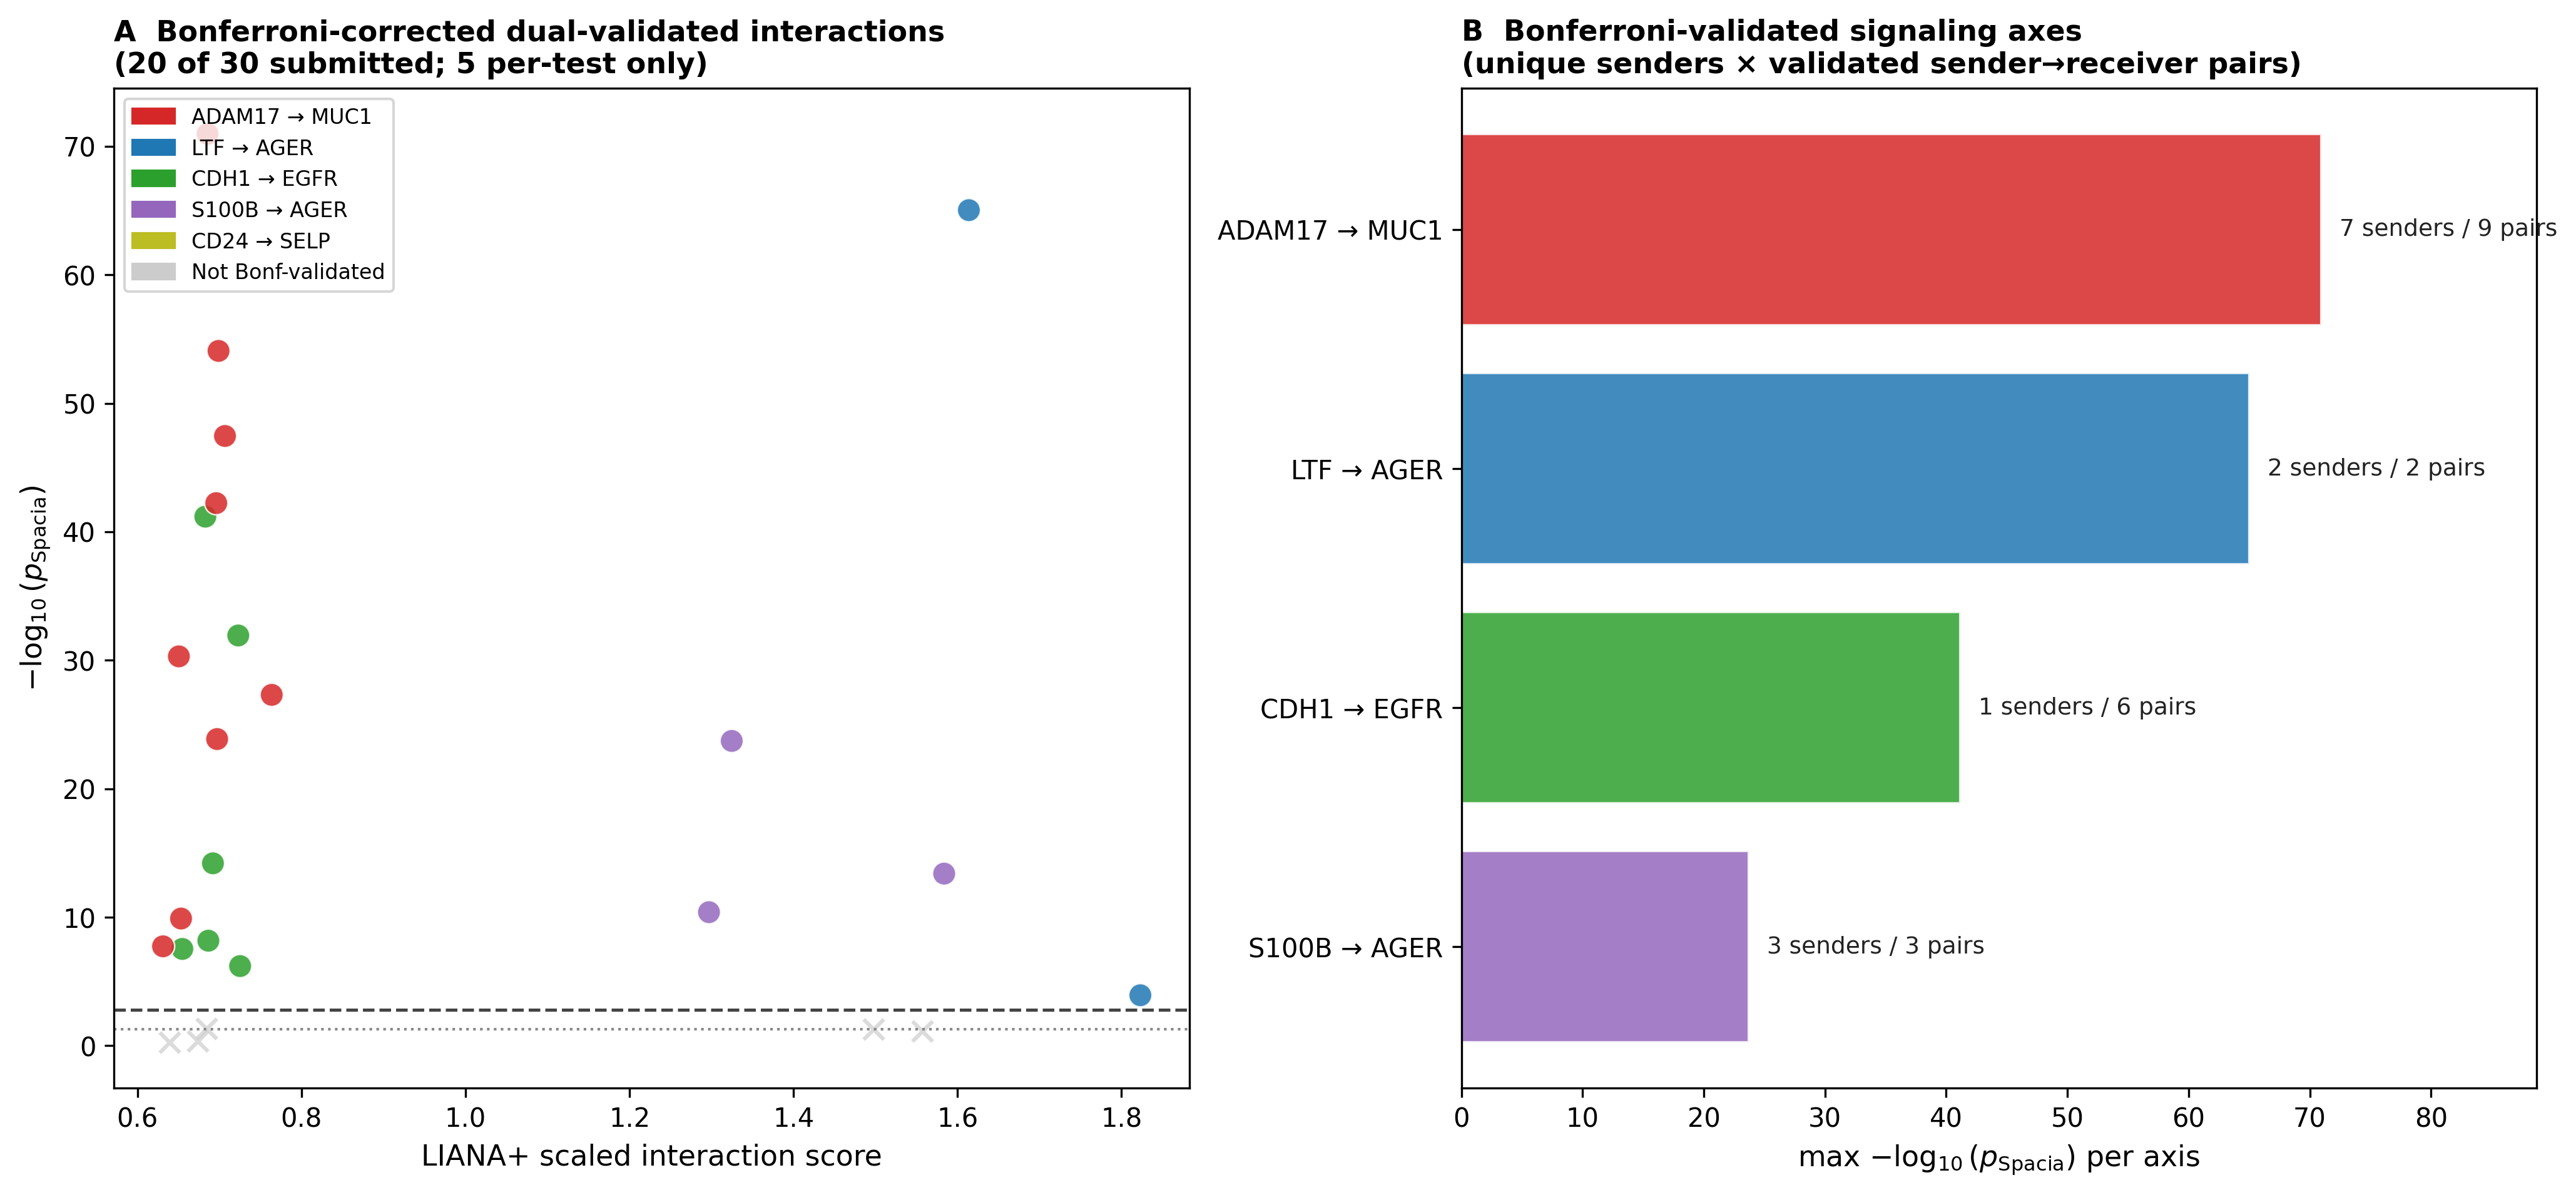
\includegraphics[width=0.95\textwidth]{figures/Fig4B_spacia_axes.png}
\caption{\textbf{Hubs de comunicación célula--célula validados espacialmente.}
\textbf{(A)} Diagrama de dispersión de las 25 interacciones Spacia completadas: el eje $y$ es $-\log_{10}(p_{\text{Spacia}})$, el eje $x$ es la puntuación escalada de LIANA+. Las cruces grises son interacciones que solo pasaron el umbral per-test pero no Bonferroni; los círculos coloreados son los 20 hubs Bonferroni-validados.
\textbf{(B)} Resumen por eje: los 4 ejes señalados por Bonferroni indicando emisores únicos y pares emisor$\to$receptor validados. ADAM17$\to$MUC1 domina con 7 emisores y 9 pares.}
\label{fig:4}
\end{figure}

\subsection*{3.5 Un continuo de activación macrofágica (no una trayectoria de polarización M1$\to$M2)}
Una primera versión de este análisis intentó aplicar Slingshot+tradeSeq a través de todos los tipos celulares principales del TME con el centroide de células tumorales proliferantes como raíz y agrupamientos inmunes/epiteliales/endoteliales como estados terminales. Discontinuamos esa estrategia porque (i) la asunción de que las células tumorales se diferencian en células T, AT1 o endoteliales no es biológicamente defendible, así que las ``trayectorias'' inferidas eran gradientes espaciales relabelados como progresión de desarrollo; y (ii) los ajustes GAM a nivel gen se aplicaron sobre dimensiones de embeddings Novae escaladas y redondeadas a enteros, lo cual viola la verosimilitud basada en counts de tradeSeq. Ambos problemas se documentan transparentemente aquí; los scripts correspondientes han sido marcados como deprecados en el repositorio público.

El análisis revisado restringe la inferencia de pseudotime al compartimento macrofágico (4,029 M1-like + 18,873 M2-like; 22,902 células totales). Se aplicaron dos métodos independientes al mismo subconjunto, ambos partiendo de la representación en componentes principales de la expresión log-normalizada de los 289 genes del panel: (i) PAGA \citep{wolf2019paga} sobre subgrupos Leiden de alta resolución, seguido de pseudotime de difusión (DPT) \citep{haghverdi2016dpt} con la raíz definida como la célula M1 más cercana al centroide del cluster M1 en espacio PCA; (ii) Slingshot \citep{street2018slingshot} con \texttt{start.clus = "Macrophage\_M1"} y sin restricción de cluster terminal. Slingshot retornó un único linaje principal abarcando las 22,902 células macrofágicas, y la correlación de rangos de Spearman entre los dos estimados de pseudotime es $r = 0.478$ ($p < 10^{-300}$, $n = 22{,}902$): los métodos coinciden en un ordenamiento grueso de las macrófagos a lo largo de un continuo pero discrepan en la escala absoluta (consistente con las diferentes métricas de distancia --- longitud de arco para Slingshot, distancia de difusión para DPT).

Críticamente, este continuo \emph{no} es un eje direccional de polarización M1$\to$M2. Probamos la direccionalidad post-hoc calculando la correlación de Spearman entre el pseudotime de Slingshot y la expresión de marcadores canónicos de polarización macrofágica disponibles en el panel de 289 genes. Si el continuo representara una verdadera polarización M1$\to$M2, los marcadores M1 (CD86, CD80, CXCL9, CXCL10) deberían disminuir y los marcadores M2 (CD163, MS4A4A, TREM2) aumentar a lo largo del pseudotime --- generando correlaciones negativas para los M1 y positivas para los M2. En cambio, \emph{ambas} clases de marcadores muestran correlaciones positivas con el pseudotime (marcadores M1: media $r = +0.34$, rango $+0.14$ a $+0.55$; marcadores M2: media $r = +0.59$, rango $+0.47$ a $+0.65$; Figura Suplementaria~S3). El eje del pseudotime parametriza por tanto el \emph{nivel global de activación macrofágica}, con los marcadores M2 mostrando incrementos mayores que los M1 a medida que la activación aumenta --- consistente con una población macrofágica reclutada por el tumor, predominantemente sesgada hacia M2, que se vuelve crecientemente activada en lugar de transicionar entre estados de polarización.

Para identificar genes del panel cuya expresión varía sistemáticamente a lo largo del continuo de activación, ajustamos modelos aditivos generalizados con tradeSeq sobre los 288 genes que sobrevivieron un filtro de suma-de-counts $>50$, usando la Lineage~1 de Slingshot como covariable de pseudotime. La prueba de asociación identifica $221$ genes (76.7\%) con expresión significativamente dependiente del continuo a $p_{\text{Bonferroni}} < 0.05$ a través de los 288 genes evaluados ($227$ genes a BH-FDR $<$ 0.05, 78.8\%). ADAM17 está entre los principales genes asociados al continuo, proveyendo consistencia interna entre este análisis y el hub de comunicación célula--célula identificado arriba. Enfatizamos que este análisis \emph{no} establece una trayectoria direccional de polarización: establece que los macrófagos en este tumor existen sobre un continuo de estados de activación, con expresión concurrente de marcadores canónicos M1 y M2 en las células más activadas. Esto es consistente con re-evaluaciones recientes de la biología macrofágica \emph{in vivo} que cuestionan la dicotomía estricta M1/M2 en tejido \citep{mantovani2022macrophage}.

\begin{figure}[htbp]
\centering
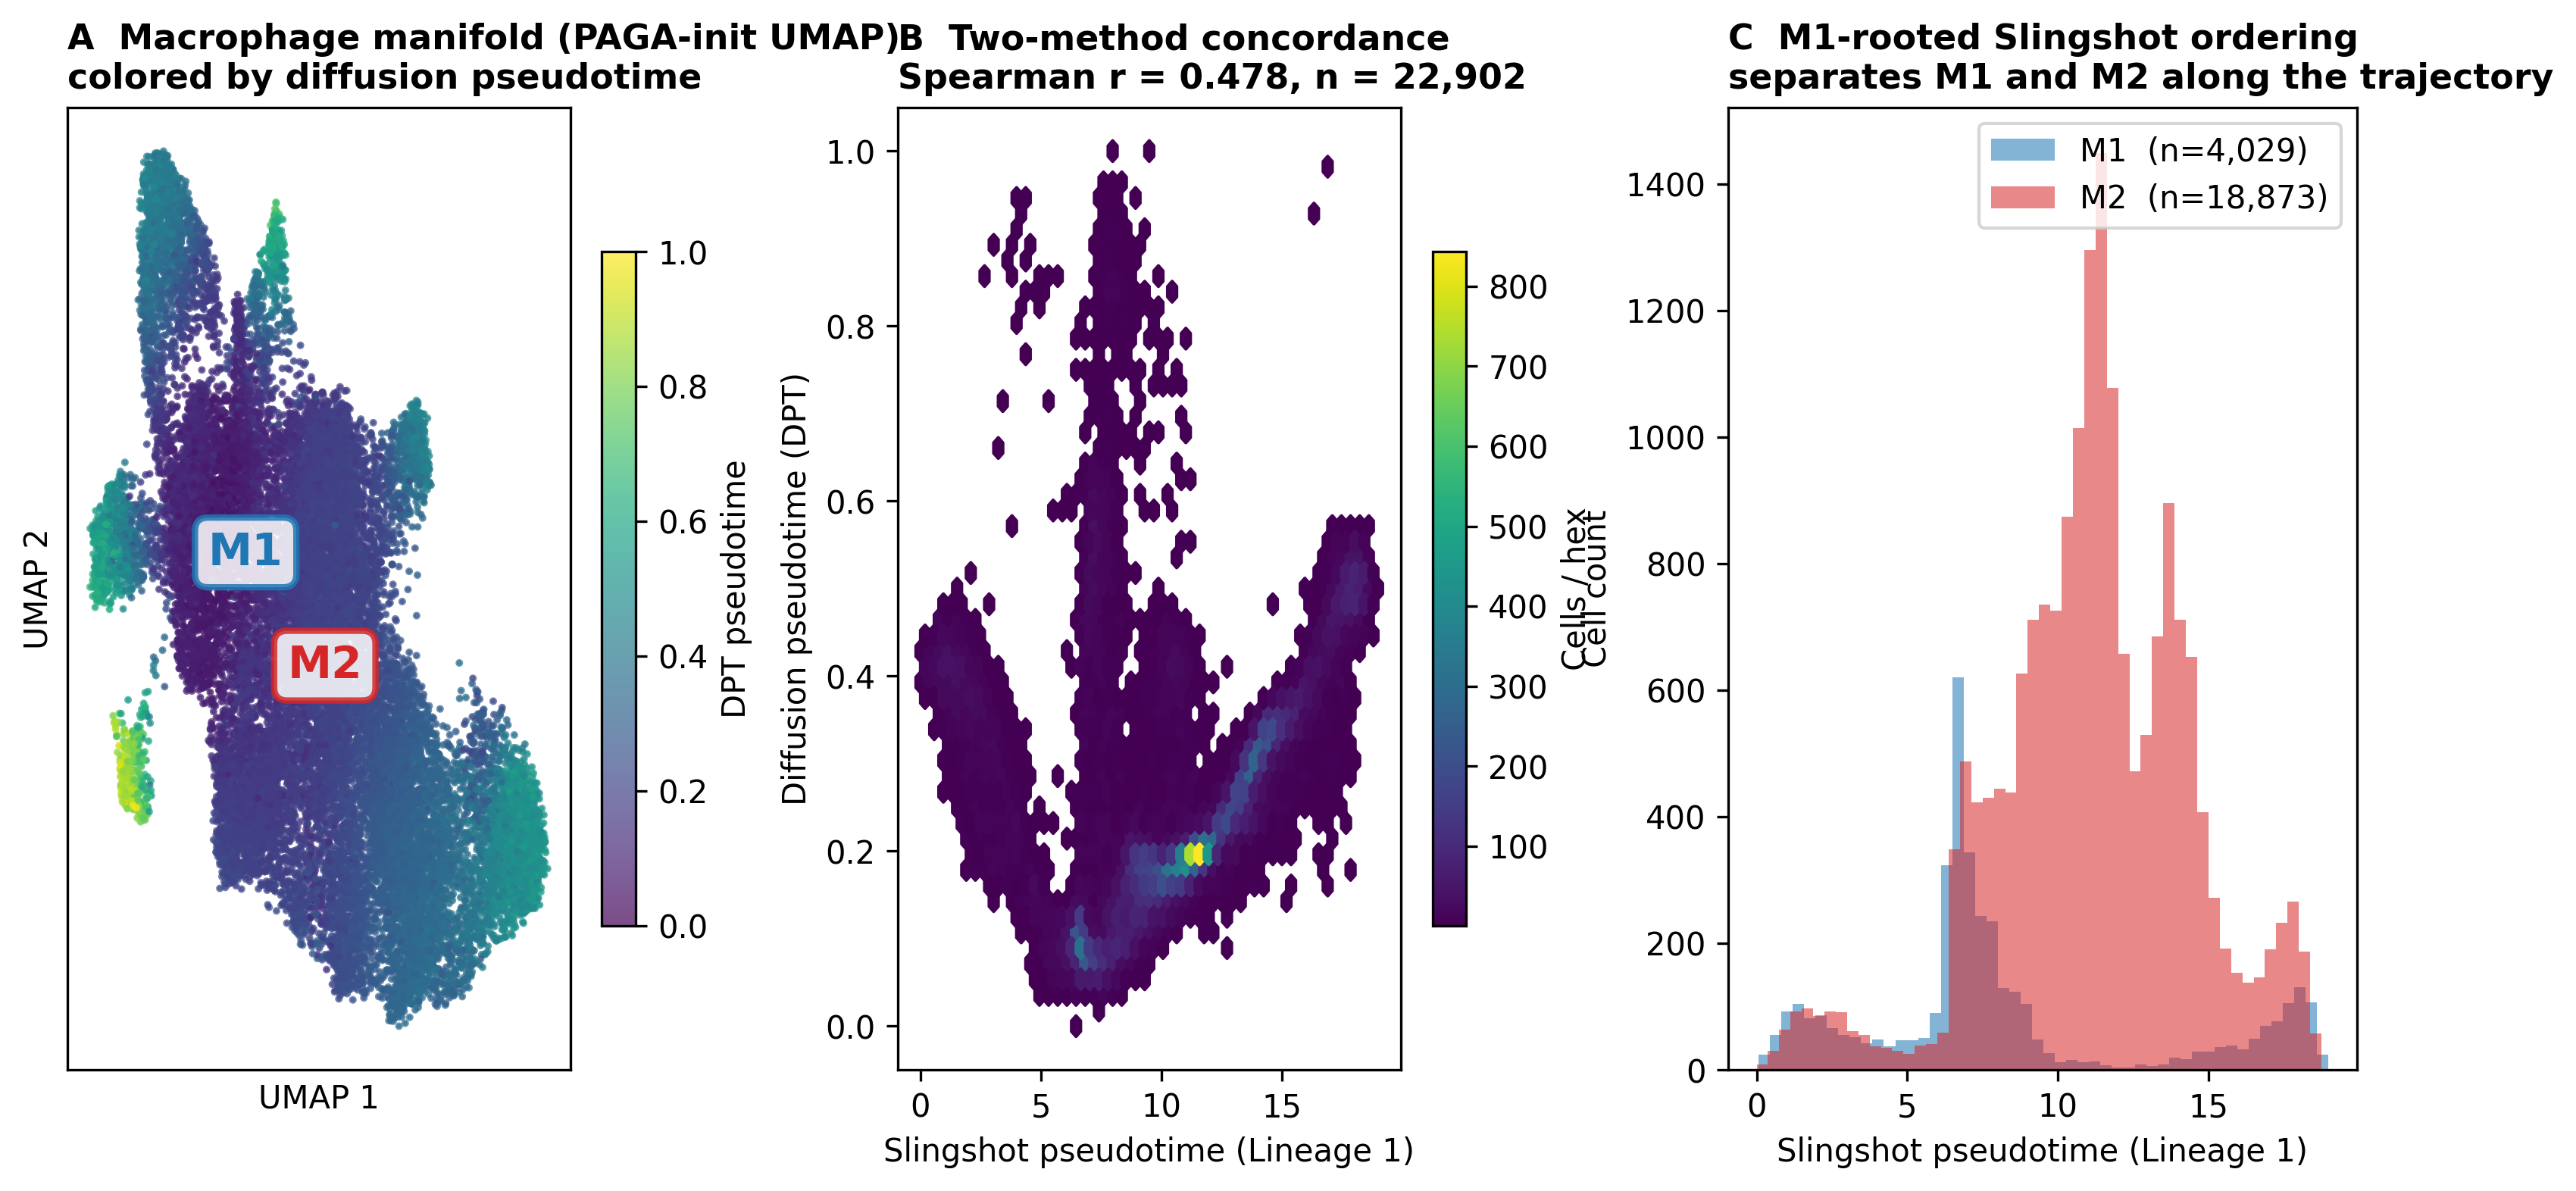
\includegraphics[width=\textwidth]{figures/Fig5B_pseudotime_proportions.png}
\caption{\textbf{Pseudotime de consenso por dos métodos sobre el continuo macrofágico.}
\textbf{(A)} Embedding UMAP de 22,902 macrófagos (4,029 M1-like, 18,873 M2-like) inicializado con PAGA \citep{wolf2019paga}, coloreado por pseudotime de difusión \citep{haghverdi2016dpt} con raíz en el centroide del cluster M1. M1 y M2 ocupan regiones distintas del manifold conectadas por estados intermedios poblados, consistente con un continuo en lugar de una dicotomía binaria.
\textbf{(B)} Densidad hexbin del pseudotime Slingshot (Lineage 1) frente al pseudotime de difusión, computado independientemente sobre las mismas células. La correlación de rangos de Spearman es $r = 0.478$ ($n = 22,902$), confirmando un ordenamiento de consenso a través de dos marcos metodológicamente distintos (difusión basada en grafo frente a ajuste de curva principal).
\textbf{(C)} Pseudotime Slingshot (con raíz en M1) por etiqueta de tipo celular: las células M1-like se concentran en valores bajos de pseudotime y las M2-like abarcan el rango medio-alto, con superposición en la región intermedia que define el continuo. Como se demuestra en el texto y Figura Suplementaria~S3, este continuo representa activación macrofágica, no polarización direccional.}
\label{fig:5}
\end{figure}

\section*{Discusión}
\label{sec:discussion}

Presentamos un marco de consenso multi-herramienta para transcriptómica espacial \textit{in situ} dirigida y demostramos su aplicación a adenocarcinoma pulmonar humano. El principio metodológico central --- retener únicamente los hallazgos confirmados por al menos dos herramientas computacionales independientes por familia analítica --- reduce sustancialmente el riesgo de reportar artefactos específicos de herramienta como hallazgos biológicos. La tasa del 80\% de validación de interacciones LIANA+ por inferencia espacial bayesiana independiente (tras corrección Bonferroni a través de los 30 tests sometidos), y la concordancia del 99.7\% de SVGs entre tres métodos de autocorrelación, sugieren que los paneles dirigidos de transcriptómica espacial portan suficiente señal para conclusiones analíticas robustas cuando múltiples métodos se aplican en paralelo, a la vez que revelan los límites cuando los métodos requieren mayor número de genes (e.g., NicheDE, hdWGCNA, SCENIC) o referencias preentrenadas (CellTypist).

El hallazgo biológico más prominente es el hub de señalización ADAM17--MUC1. ADAM17 (también conocida como TACE) es una sheddasa que procesa los ectodominios de TNF-$\alpha$, TGF-$\alpha$, ligandos del EGFR y múltiples otros sustratos \citep{lambrecht2018adam17}. Su actividad en células mieloides --- particularmente macrófagos --- ha sido vinculada a liberación de citocinas inmunosupresoras y remodelación estromal pro-tumoral. MUC1, el receptor, es una oncomucina cuyo dominio intracelular activa señalización NF-$\kappa$B y Wnt en células tumorales y cuyo dominio extracelular bloquea físicamente la unión efector inmune \citep{nath2013muc1}. Nuestros datos revelan que este eje está activo tanto en macrófagos M1- como M2-like, sugiriendo que no depende de un contexto específico de polarización sino que representa una característica constitutiva de la interfaz macrófago--célula tumoral. Este hallazgo extiende la evidencia in vitro de co-actividad ADAM17--MUC1 a tejido espacial FFPE intacto y motiva la evaluación terapéutica de inhibidores de ADAM17 en combinación con agentes de checkpoint, sujeto a validación en cohortes.

Los análisis de dominios espaciales y pseudotime convergen en un motivo anatómico consistente: una zona intermedia enriquecida en mieloides entre el parénquima alveolar sano y el núcleo tumoral. Esta arquitectura espacial es distinta de los arquetipos de TME ``desierto inmune'' o ``inflamado'' definidos en transcriptómica de volumen \citep{chen2016elements}. El enriquecimiento de macrófagos M2-like y monocitos en el margen tumoral, en lugar de células T o NK, identifica esta muestra como un TME inmuno-excluido o mieloide-suprimido, asociado con peor pronóstico y respuesta reducida a inmunoterapia de checkpoint en adenocarcinoma pulmonar \citep{cassetta2020targeting, wu2021single}.

Varias limitaciones de este estudio merecen discusión. Primero, el análisis se basa en una sola sección de tejido de un paciente. La resolución a nivel de célula ofrece alto poder estadístico para inferencia espacial dentro de la sección, pero cada célula no es un replicado biológico independiente: los $p$-valores bayesianos altamente significativos reportados (hasta $1.10 \times 10^{-71}$) reflejan co-localización espacial dentro de este espécimen y no se generalizan \emph{ipso facto} a una población de pacientes. Si el hub ADAM17--MUC1 y el nicho intermedio mieloide enriquecido son características recurrentes del adenocarcinoma pulmonar --- en oposición a características específicas de este espécimen acinar invasivo Estadio IB --- requiere validación en cohortes; este estudio se interpreta mejor como un caso metodológico + demostración de marco, acompañado por observaciones biológicas generadoras de hipótesis. Segundo, el panel Xenium de 289 genes precluyó análisis de factores de transcripción, ARNs no codificantes y muchos checkpoints inmunes; en particular, métodos diseñados para datos de transcriptoma completo (NicheDE, hdWGCNA, SCENIC, mapeo a referencia con CellTypist) colapsaron a salidas no informativas en el panel dirigido y no fueron retenidos en el marco de consenso, con esta exclusión documentada transparentemente en lugar de enmascarada. Métodos espaciales de transcriptoma completo (Visium HD, MERFISH a $\geq$1,000 genes) serían necesarios para recuperar esos análisis. Tercero, la tasa del 99.7\% de SVG-consenso refleja parcialmente el sesgo de selección del panel; un panel control no preseleccionado por especificidad espacial sería necesario para calibrar el verdadero poder discriminativo del marco de SVG. Cuarto, el marco de consenso opera al nivel de coincidencia entre métodos independientes dentro de una familia analítica; la coincidencia no implica por sí sola causalidad mecanística, y varios pares CCC validados (notablemente ADAM17--MUC1) son no canónicos en el sentido estricto receptor--ligando y requieren seguimiento funcional. Quinto, la química FFPE introduce fragmentación de transcritos que puede afectar la detección de genes de baja abundancia; la concordancia de hallazgos SVG entre tres métodos sugiere que este artefacto no domina nuestras conclusiones pero no puede excluirse para interacciones individuales raras.

El trabajo futuro aplicará este pipeline de consenso a una cohorte en tissue microarray de 28 donadores --- 16 en un panel Xenium pulmonar (10 con fibrosis pulmonar asociada a desórdenes de biología telomérica más 6 controles no-enfermedad estratificados por longitud telomérica y por estatus neoplásico) y 12 en un panel hepático paralelo (4 con fibrosis hepática asociada a desórdenes de biología telomérica, 4 con cirrosis alcohólica como comparador fibrótico no-telomérico, y 4 controles sanos) --- utilizando dos paneles Xenium de 439 genes enfocados en inmunidad y fibrosis. El diseño de dos tejidos con tres niveles de condición introducirá tanto la replicación biológica que este piloto carece como el contraste (fibrosis telomérica vs.\ cirrosis alcohólica) que distingue firmas fibróticas telómero-específicas de fibrosis genérica. El marco está diseñado para acomodar la integración multi-muestra: cada módulo analítico se implementa como una regla de flujo de trabajo independiente con checkpoints explícitos de generizidad de panel (Métodos suplementarios; checklist de portabilidad del pipeline en el repositorio de código), permitiendo adaptación plug-and-play a diferentes paneles y contextos de enfermedad a medida que el campo avanza.

\section*{Métodos}
\label{sec:methods}

\subsection*{Conjunto de datos y preprocesamiento}
Analizamos un conjunto de datos público de Xenium \textit{in situ} de adenocarcinoma pulmonar humano (10x Genomics, accession CG000709 Rev C). El tejido se obtuvo de un bloque FFPE (Avaden Biosciences) de adenocarcinoma acinar invasivo Estadio IB (T2a N0 MX). El perfilado de expresión génica utilizó el Xenium Human Lung Gene Expression Panel v1.1 (289 genes objetivo más 87 sondas de control negativo). Se ejecutó Xenium Onboard Analysis v3.0.0 en el instrumento para producir las salidas de segmentación celular y asignación de transcritos.

Se aplicó control de calidad para remover células con menos de 5 transcritos, área celular mayor a 1,500~$\mu$m$^{2}$ y sondas de control negativo. Un total de 268,034 células pasaron el filtrado de las 278,659 detectadas (96.2\% de retención). Los counts de transcritos se normalizaron usando \texttt{scanpy} \citep{wolf2018scanpy}: normalización por tamaño de librería a 10,000 counts por célula, seguido de transformación $\log_{1p}$. Los counts crudos se retuvieron en una capa separada para herramientas que requieren input entero. Todos los datos se almacenaron en formato SpatialData Zarr usando \texttt{spatialdata} \citep{marconato2024spatialdata}.

\subsection*{Anotación de tipos celulares}
La anotación siguió una estrategia híbrida de tres fuentes. Primero, las células inmunes se identificaron por subagrupamiento iterativo: las poblaciones inmunes amplias se aislaron por expresión de marcadores canónicos disponibles en el panel y luego se reagruparon a mayor resolución para resolver subtipos mieloides y linfoides. Segundo, las 268,034 células se sometieron a detección de comunidades Leiden a múltiples resoluciones ($\gamma = 0.3$, $0.5$, $0.8$) sobre un grafo de vecinos compartidos construido a partir de los 30 primeros componentes principales de la expresión log-normalizada, y las etiquetas de comunidad se asignaron al tipo celular conocido con mayor puntuación usando \texttt{scanpy.tl.score\_genes}. Tercero, un enfoque de puntuación con firmas génicas curadas (3--12 marcadores por tipo derivados de atlas pulmonares e inmunes publicados \citep{travaglini2020molecular}) resolvió células ambiguas. Las células con puntuación bajo el umbral en todas las firmas se etiquetaron como Unassigned (4.8\% de las células). La taxonomía final comprende 14 categorías amplias, 26 subtipos granulares y 7 estados funcionales. La concordancia se evaluó calculando el ARI entre la anotación primaria y un subagrupamiento computacional independiente de células inmunes, reportando ARI = 0.742 como métrica de estabilidad interna.

\subsection*{Identificación de genes espacialmente variables}
Se aplicaron tres métodos para identificar SVGs. Hotspot \citep{detomaso2021hotspot} v1.1.3 calculó estadísticas de autocorrelación local para cada gen usando un modelo de vecindario con kernel gaussiano; se retuvieron los genes con $Z$-score $> 1.96$. nnSVG \citep{weber2023nnsvg} v1.12 ajustó modelos de proceso gaussiano no paramétrico basados en rangos sobre una submuestra aleatoria de 10,000 células (seed = 42); se retuvieron los genes con FDR $<$ 0.05. Moran's~I se calculó usando \texttt{squidpy.gr.spatial\_autocorr} \citep{palla2022squidpy} sobre un grafo de $k$ vecinos más cercanos ($k=6$); se retuvieron los genes con $p$ corregido $<$ 0.05 (Benjamini--Hochberg). Un gen se declaró SVG de consenso si fue significativo en al menos dos de los tres métodos. Se evaluaron los 289 genes; 288 (99.7\%) cumplieron el criterio de consenso.

\subsection*{Inferencia de dominios espaciales}
La inferencia de dominios usó dos enfoques independientes. Novae \citep{schaar2025novae} (modelo: novae-human-0, MICS-Lab) se aplicó con hiperparámetros por defecto, produciendo embeddings latentes de 64 dimensiones por célula que se agruparon en 10 dominios amplios (etiquetas D971, D985, D998, D1000, D1004, D1006, D1008, D1010, D1012, D1013). Banksy \citep{zhao2023banksy} se ejecutó con parámetro de agregación de vecindario $\lambda = 0.2$, vecindario geométrico $k_{\text{geom}} = 6$, y detección de comunidades Leiden con $\gamma = 0.5$, generando 14 dominios finos (B1--B14). La concordancia a nivel de partición se evaluó por el adjusted Rand index (ARI~$=0.15$) y la información mutua normalizada (NMI~$=0.31$) calculadas sobre el conjunto conjunto de etiquetas de las 268,033 células. Se definió adicionalmente una asignación estricta de consenso por célula como el subconjunto de células para el que el dominio Banksy de la célula tiene un mejor-match Novae inequívoco ($\geq 50\%$ de las células del dominio Banksy residiendo en ese dominio Novae) y la propia célula está asignada a ese dominio Novae; 94,869 células (35.4\%) cumplieron este criterio estricto (Figura Suplementaria~S2).

\subsection*{Análisis de comunicación célula--célula}
La CCC se analizó en dos etapas. Primero, LIANA+ \citep{ramirez2024liana} v1.7.1 se ejecutó usando el método de consenso \texttt{rank\_aggregate}, que agrega $p$-valores y rangos de CellChat \citep{jin2021inference}, CellPhoneDB \citep{efremova2020cellphonedb}, NATMI \citep{hou2020predicting}, Connectome y scSeqComm. El análisis usó 1,000 permutaciones, el recurso de consenso ligando--receptor, un radio espacial de 200~$\mu$m, y ponderación bivariada de coseno. Los $p$-valores del componente CellPhoneDB (\texttt{cellphone\_pvals} en la salida de LIANA+) se retuvieron como el $p$-valor por interacción y se ajustaron a través de las 2,631 combinaciones emisor--receptor--ligando--receptor usando Benjamini--Hochberg, generando 1,557 interacciones a BH-FDR $<$ 0.05. Las 30 interacciones de mayor magnitud por consenso de LIANA+ se seleccionaron para la validación espacial de segunda etapa.

Segundo, Spacia \citep{zhu2024spacia} se aplicó a cada una de las 30 interacciones candidatas usando las coordenadas espaciales completas y la expresión normalizada por célula. Spacia emplea aprendizaje por instancias múltiples bayesiano con muestreo MCMC (50,000 iteraciones totales, 20,000 burn-in, intervalo de adelgazamiento 100, 2 cadenas) para estimar si el arreglo espacial de pares emisor--receptor es consistente con señalización direccional. Se utilizó un cutoff espacial de vecindario de 30~$\mu$m (rango típico de la señalización yuxtacrina directa célula--célula), y cada tipo celular se submuestreó a un máximo de 5,000 células por tipo para tractabilidad. Para complejos de ligando y receptor con múltiples subunidades, se utilizó el primer gen listado como característica de prueba (limitación conocida del análisis con Spacia sobre complejos multi-subunidad). De las 30 interacciones sometidas, 5 fallaron porque el tipo emisor contenía menos de 500 células (interacciones con Plasma, Plasmablast, DC madura y pDC), dejando 25 con ajustes bayesianos completos. Una interacción se declaró validada dualmente si (i) fue retenida a LIANA+ Benjamini--Hochberg FDR $<$ 0.05 sobre \texttt{cellphone\_pvals}, \emph{y} (ii) el $p$-valor per-test de Spacia sobrevivió la corrección Bonferroni a través de los 30 tests sometidos ($p < 1.67 \times 10^{-3}$). Bajo este criterio dual, 20 de las 30 sometidas (67\%; 20 de las 25 completadas, 80\%) fueron retenidas. Las dos interacciones que perdieron significancia bajo Bonferroni respecto al umbral per-test (cDC1$\to$Tumor\_resting vía ADAM17--MUC1, $p=0.048$; Ciliated$\to$Endothelial\_blood vía CD24--SELP, $p=0.049$) estaban ambas en el margen de la significancia per-test.

\subsection*{Análisis de pseudotime (continuo macrofágico)}
La inferencia de pseudotime se restringió al compartimento macrofágico (células anotadas como Macrophage\_M1 o Macrophage\_M2 en la taxonomía L2; 22,902 células totales). Se aplicaron dos métodos independientes al mismo input.

Para PAGA + DPT, la expresión log-normalizada de los 289 genes del panel se redujo a 30 componentes principales en scanpy 1.11.5 \citep{wolf2018scanpy}; se construyó un grafo de $k$ vecinos más cercanos ($k = 15$) y un subagrupamiento Leiden ($\gamma = 0.5$, seed = 42) generó 11 subclusters macrofágicos. Se calculó PAGA \citep{wolf2019paga} sobre el grafo de subclusters, se utilizó como inicialización para un UMAP, y el pseudotime de difusión \citep{haghverdi2016dpt} se calculó con la célula raíz definida como la célula etiquetada M1 más cercana al centroide del cluster M1 en espacio PCA.

Para Slingshot, la misma matriz PCA se cargó en R (R 4.5.3, Bioconductor 3.22, slingshot 2.16) como entrada de dimensión reducida, con etiquetas de cluster = \texttt{cell\_type\_L2}, \texttt{start.clus = "Macrophage\_M1"}, sin restricción de cluster terminal, y \texttt{approx\_points = 150}. Slingshot retornó un único linaje de curva principal; el pseudotime de longitud de arco se extrajo de \texttt{slingPseudotime\_1}.

La concordancia entre los dos estimados se cuantificó por correlación de rangos de Spearman a través de las 22,902 macrófagos. La direccionalidad se evaluó post-hoc calculando la correlación de Spearman entre el pseudotime y la expresión de marcadores canónicos M1 (CD86, CD80, CXCL9, CXCL10) y M2 (CD163, MS4A4A, TREM2) presentes en el panel; ambas clases mostraron correlaciones positivas con el pseudotime, indicando que el continuo parametriza activación global en lugar de polarización direccional. Las dinámicas a nivel de gen a lo largo del Lineage~1 se estimaron con tradeSeq \citep{vandenberge2020tradeseq} fitGAM (GAMs binomiales negativas, $k = 6$ knots, backend BiocParallel paralelo con 2 workers) sobre los 288 genes del panel que sobrevivieron un filtro de suma-de-counts $> 50$; los $p$-valores de la prueba de asociación se corrigieron por Bonferroni a través de los 288 genes evaluados. El análisis previo de pseudotime sobre el manifold Tumor$\to$multi-end ha sido removido del manuscrito presente y el script correspondiente (\texttt{F5\_pseudotime\_slingshot.R}) está deprecado en el repositorio público porque (i) impuso una configuración raíz--terminal de desarrollo no plausible sobre Slingshot y (ii) aplicó el GAM basado en counts de tradeSeq a dimensiones de embeddings Novae escaladas y redondeadas, ambas no soportadas por los métodos subyacentes.

\subsection*{Software y reproducibilidad}
Todos los análisis se orquestaron mediante un workflow Snakemake \citep{molder2021snakemake} que captura el grafo acíclico de dependencias y fija las versiones de las herramientas por etapa en entornos conda dedicados. Todos los análisis en Python se ejecutaron en un entorno conda dedicado conteniendo spatialdata 0.7.2, scanpy 1.11.5, anndata 0.12.10, liana 1.7.1, novae 1.0.5, hotspotsc 1.1.3, squidpy 1.8.1 y celltypist 1.7.1. Los análisis en R utilizaron un entorno conda separado basado en Bioconductor 3.22: slingshot 2.16, tradeSeq 1.22, nnSVG 1.12 y Banksy 1.6.0 (implementación R/Bioconductor; no se utilizó Python Banksy). Spacia (commit de \url{https://github.com/JianingTangBigData/Spacia} clonado localmente; no empaquetado en PyPI) se ejecutó vía el script de entrada \texttt{spacia.py} en un entorno conda de Python 3.8 separado con numpy 1.24.3, pandas 2.0.3 y R 4.5.3 utilizado internamente para el ajuste bayesiano. Las rutas hardcoded en la implementación actual serán parametrizadas para la versión pública; en el ínterin, el entorno completo está capturado en archivos \texttt{environment.yml} y se provee una receta Docker (\texttt{Dockerfile}) y Singularity (\texttt{singularity\_build.def}) para Spacia. Las figuras se generaron usando matplotlib \citep{hunter2007matplotlib}, seaborn y los colormaps perceptualmente uniformes de Crameri \citep{crameri2023scientific}. El código de análisis está disponible en \url{https://github.com/MiguelDiaz02/xenium-spatial-transcriptomics}; la versión auditada y refactorizada está etiquetada para la fecha de submission. El conjunto de datos está públicamente disponible en el sitio de 10x Genomics (CG000709 Rev C).

\section*{Disponibilidad de datos}
El conjunto de datos analizado en este estudio está públicamente disponible en el sitio de 10x Genomics bajo el accession CG000709 Rev C.

\section*{Disponibilidad de código}
Todos los scripts de análisis están disponibles en \url{https://github.com/MiguelDiaz02/xenium-spatial-transcriptomics}.

\section*{Agradecimientos}
Agradecemos al Instituto Nacional de Pediatr\'{i}a y al Instituto de Investigaciones Biom\'{e}dicas (UNAM) por proveer recursos institucionales e infraestructura computacional. Información de financiamiento: pendiente.

\section*{Contribuciones de los autores}
M.A.D.-C.: Conceptualización, metodología, software, análisis formal, curación de datos, redacción del borrador original. A.R.G.: Supervisión, revisión y edición, adquisición de fondos, recursos.

\section*{Intereses en conflicto}
Los autores declaran no tener intereses en conflicto.

\bibliographystyle{unsrtnat}
\bibliography{refs}

%% ===== SUPLEMENTARIO =====
\newpage
\setcounter{section}{0}
\renewcommand{\thesection}{S\arabic{section}}
\renewcommand{\thefigure}{S\arabic{figure}}
\setcounter{figure}{0}
\section*{Información Suplementaria}

\subsection*{Nota S1 --- Decisiones metodológicas y memorando de auditoría}

\noindent\textit{Este memorando resume las razones detrás de las decisiones metodológicas reportadas en el texto principal, la auditoría posterior que motivó varias de las correcciones, y la ruta planeada hacia la portabilidad del pipeline para cohortes futuras. Su propósito es ofrecer a revisores y colaboradores una vista transparente del árbol de decisiones detrás del marco metodológico.}

\paragraph{S1.1 Métodos descartados por restricciones del panel génico.}
El panel Xenium v1 utilizado contiene 289 genes dirigidos. Varios métodos fueron evaluados y descartados por inaplicabilidad a esta escala:
\begin{itemize}
    \item \textbf{NicheDE} --- requiere expresión a nivel de transcriptoma para modelar expresión diferencial a nivel de vecindario espacial; con 289 genes el poder estadístico colapsa. Descartado.
    \item \textbf{hdWGCNA y SCENIC} --- la inferencia de redes de coexpresión y de regulones requiere miles de genes para identificar módulos/regulones estables. Descartados.
    \item \textbf{CellTypist} --- preentrenado sobre referencias scRNA-seq de transcriptoma completo ($\sim$20{,}000 genes); aplicado a un panel de 289 genes colapsa a 4--5 clases amplias independientemente del modelo de referencia (\texttt{Human\_Lung\_Atlas}, \texttt{PF/IPF\_Lung}, \texttt{Immune\_All\_High/Low}, todos probados). Ejecutado por completitud; no usado como validador externo.
\end{itemize}

\paragraph{S1.2 Elecciones metodológicas para los análisis retenidos.}
\begin{itemize}
    \item \textbf{LIANA+ \texttt{rank\_aggregate}} consensúa cinco esquemas de score (CellPhoneDB, NATMI, Connectome, SingleCellSignalR, logFC) y reduce el sesgo de un único método. El filtro previo ``FDR $<$ 5\%'' era en realidad un corte por rango de magnitud; se reemplazó por FDR Benjamini--Hochberg sobre los p-values de CellPhoneDB (1{,}565 $\to$ 1{,}557 pares significativos).
    \item \textbf{Spacia (MIL Bayesiano)} fue seleccionado para validación espacial de las predicciones de LIANA+ porque modela explícitamente la proximidad espacial y entrega probabilidades posteriores por par. Se aplicó corrección de Bonferroni sobre los 30 tests cruzados sometidos (por test $p < 1.67 \times 10^{-3}$); 20 de 30 ejes sobrevivieron.
    \item \textbf{Slingshot + DPT (pseudotiempo dual)} reemplazó un pipeline previo de Slingshot únicamente que aplicaba tradeSeq sobre embeddings de Novae forzados a counts enteros, violando la verosimilitud binomial-negativa. El pipeline corregido usa counts crudos sobre M1+M2 ($n=22{,}902$ células), reportando concordancia entre Slingshot y DPT (Spearman $r=0.478$).
    \item \textbf{Banksy + Novae (inferencia dual de dominios espaciales)} captura escalas complementarias: Banksy resuelve 14 dominios finos, Novae captura 10 compartimentos amplios (ARI $=0.151$, NMI $=0.309$). El 35.4\% de consenso por célula se reporta como filtro estricto, no como evidencia de redundancia.
\end{itemize}

\paragraph{S1.3 Reformulación de paper biológico a marco metodológico + caso de estudio.}
Una auditoría tipo revisor identificó cinco problemas bloqueantes para publicación en el encuadre original (paper biológico):
\begin{enumerate}
    \item tradeSeq aplicado sobre embeddings de Novae (estadísticamente inválido).
    \item Slingshot con \texttt{start.clus} = \texttt{Tumor\_proliferating} y endpoints mezclando inmunidad, epitelio y endotelio (trayectoria biológicamente implausible).
    \item ``FDR $<$ 5\%'' de LIANA+ era en realidad top-$K$ por rango, no FDR.
    \item ``22 de 25 = 88\% validados'' de Spacia usaba p-values por test sin corrección cross-test.
    \item Versiones de software, parámetros MCMC y umbrales de submuestreo reportados en el manuscrito no coincidían con el código ejecutado.
\end{enumerate}
Junto con las restricciones inherentes a un caso de estudio con $n=1$ paciente sobre un panel dirigido de 289 genes, estos problemas motivaron reformular el manuscrito como un \textit{marco de consenso multi-método con una demostración piloto}. Título, resumen y discusión fueron reescritos en consecuencia; los hallazgos (p.\ ej., el hub ADAM17--MUC1) se reportan como candidatos del caso de estudio, no como biología generalizable.

\paragraph{S1.4 Límites de interpretación explicitados.}
\begin{itemize}
    \item \textbf{$n=1$ paciente.} Los p-values a nivel de célula que alcanzan $10^{-71}$ no son p-values de réplica biológica; los hallazgos son generadores de hipótesis.
    \item \textbf{Sesgo por selección de panel.} La tasa de 99.7\% de genes espacialmente variables es consistente con un panel deliberadamente enriquecido en marcadores tejido-restringidos; se requiere comparación contra housekeeping o genes aleatorios no expresados para calibrar el poder discriminativo.
    \item \textbf{ADAM17--MUC1 no es canónico.} ADAM17 es una sheddasa, MUC1 una mucina transmembrana; el par está en la base de conocimiento de LIANA+ pero su interpretación como eje de señalización directa permanece tentativa.
\end{itemize}

\paragraph{S1.5 Infraestructura de reproducibilidad.}
El entorno conda original de Spacia contenía esencialmente sólo \texttt{numpy}, \texttt{pandas} y \texttt{r-base}, con el binario de Spacia invocado desde un clone manual del repositorio --- rompiendo la reproducibilidad. Se construyó una imagen Docker (\texttt{spacia:audited}, 4.4 GB) que empaqueta el pipeline completo de Spacia; una receta Singularity está planeada para uso en HPC.

\paragraph{S1.6 Ruta hacia la cohorte de desórdenes de biología telomérica.}
Un segundo conjunto de datos está siendo recolectado para análisis con el mismo marco: dos láminas Xenium en formato tissue microarray (una pulmonar, una hepática) que alojan 28 donadores en total, procesadas con dos paneles órgano-específicos de 439 genes (pulmón e hígado). El TMA pulmonar contiene 16 donadores --- 10 con fibrosis pulmonar asociada a desórdenes de biología telomérica más 6 controles no-enfermedad estratificados por longitud telomérica (telómero no-corto) y por estatus neoplásico (no-neoplásico) --- y el TMA hepático contiene 12 donadores --- 4 con fibrosis hepática asociada a desórdenes de biología telomérica, 4 con cirrosis alcohólica como comparador fibrótico no-telomérico, y 4 controles sanos. Cada donador está representado por varios cores de réplica técnica ($\geq 3$); la unidad de replicación estadística es el donador y la unidad de inferencia espacial es el core. La adaptación del pipeline actual requiere por tanto (i) externalización de paths cableados y de marcadores tejido-específicos (\textbf{P0}: completo), (ii) parametrización de umbrales de QC y clustering (\textbf{P0}: completo), (iii) integración multi-muestra consciente del TMA vía scVI con muestra-como-core y donador-como-covariable-categórica (\textbf{P1}: completo), (iv) expresión diferencial pseudobulk a nivel de donador con dos métodos (decoupler + muscat con reporte de consenso; \textbf{P1}: completo), y (v) Spacia por core seguido de meta-análisis a nivel de donador y de condición (\textbf{P1}: scaffolded). El trabajo de portabilidad se está priorizando sobre refinamientos metodológicos adicionales (p.\ ej., comparación SVG nulo, benchmarks sintéticos contra pares ligando--receptor con ground-truth) porque la fecha de llegada de la cohorte es fija y el contraste analítico que distingue la fibrosis telomérica de la cirrosis alcohólica requiere que la maquinaria de contraste multi-muestra esté operativa desde el día 1.

\subsection*{Figura Suplementaria 1 --- Métricas de control de calidad}
\begin{figure}[h!]
\centering
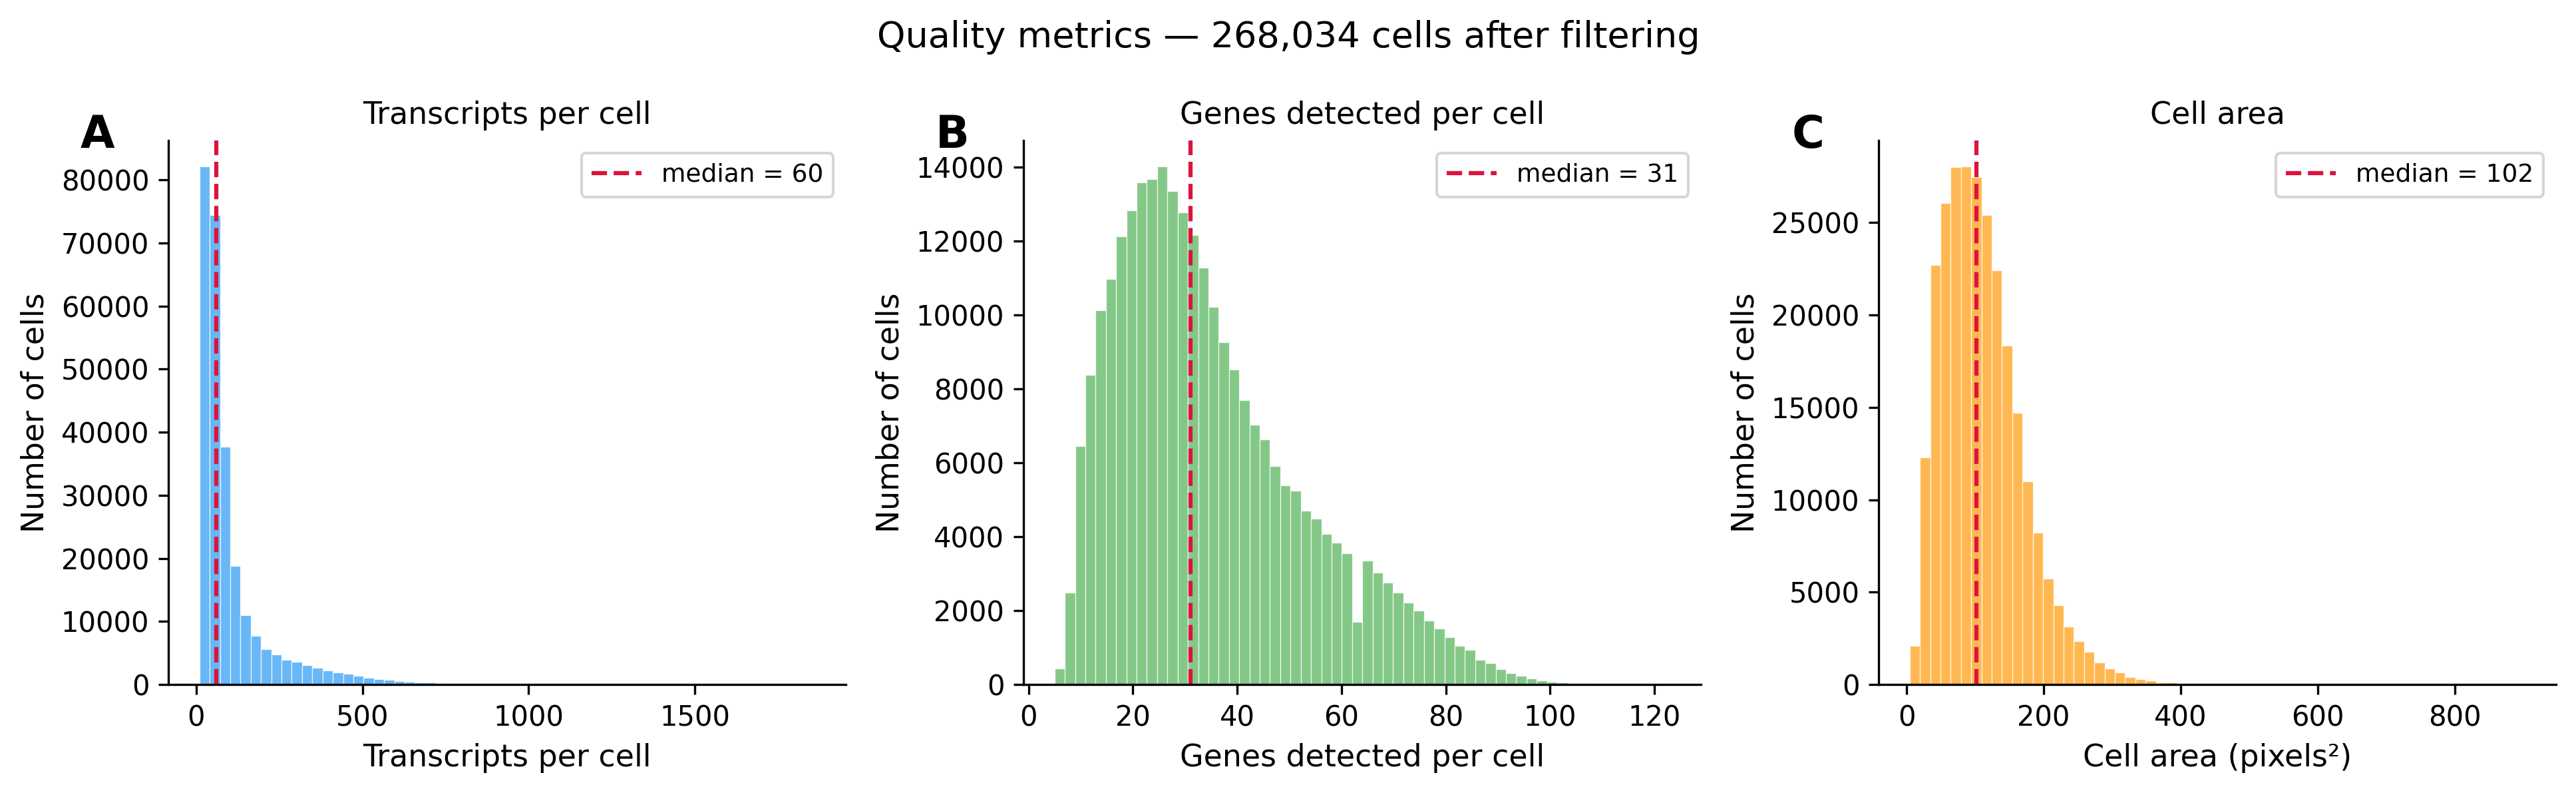
\includegraphics[width=\textwidth]{figures/FigS1_qc_metrics.png}
\caption{\textbf{Métricas de control de calidad.} Distribución de counts de transcritos por célula, genes detectados y área celular antes y después del filtrado. Umbrales aplicados: counts $\geq$5, área celular $\leq$1,500~\textmu m$^{2}$. Un total de 268,034 células pasaron el control de calidad de las 278,659 detectadas.}
\label{fig:s1}
\end{figure}

\subsection*{Figura Suplementaria 2 --- Matriz de confusión entre dominios espaciales de Banksy y Novae}
\begin{figure}[h!]
\centering
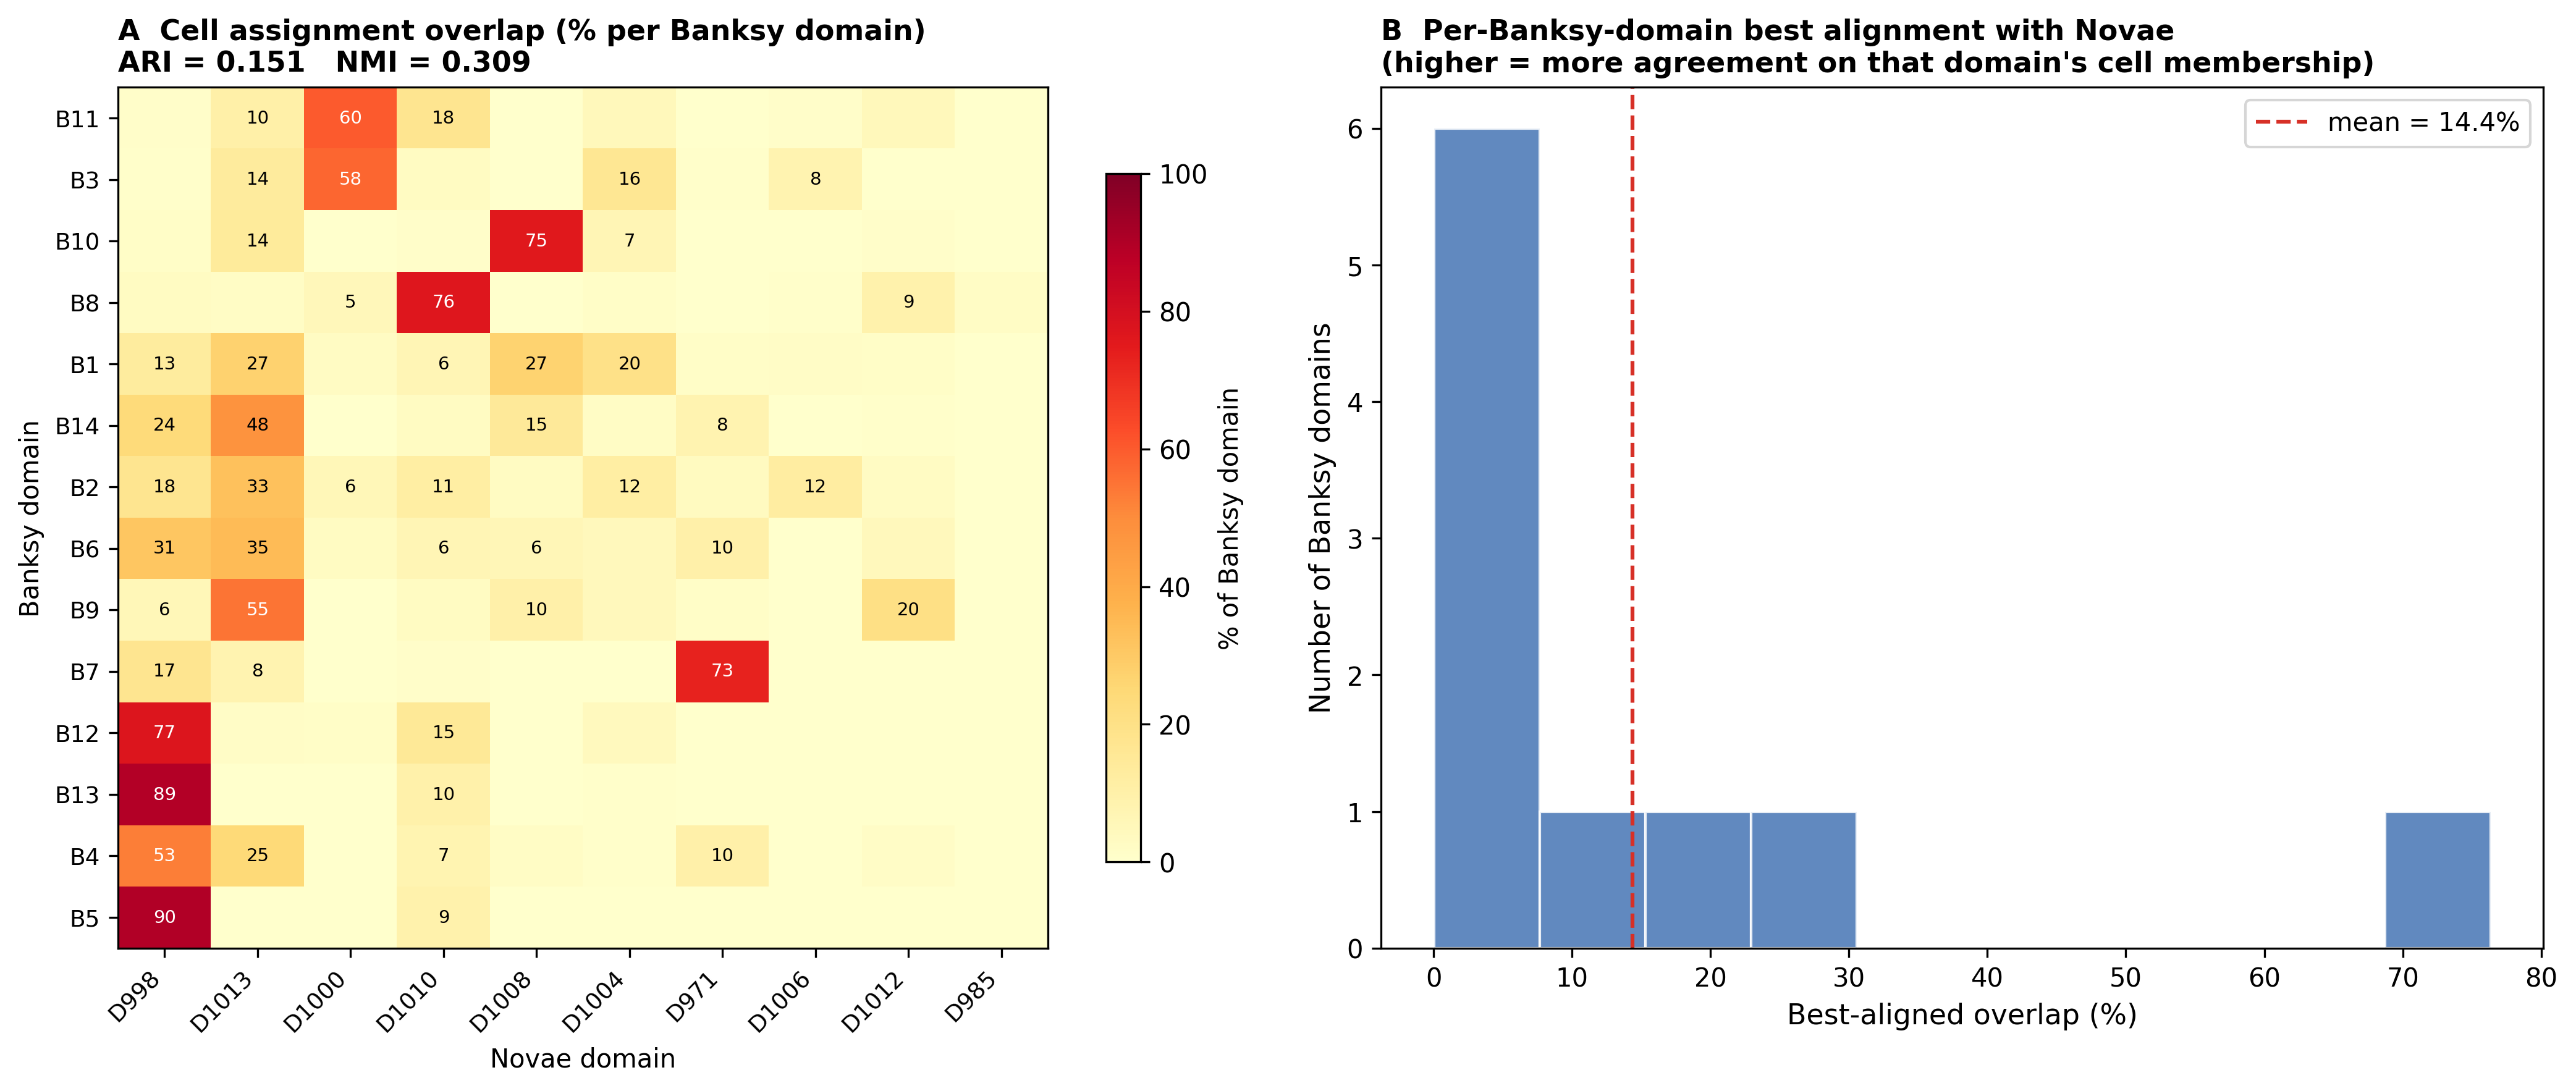
\includegraphics[width=0.85\textwidth]{figures/FigS2_banksy_novae_confusion.png}
\caption{\textbf{Matriz de confusión entre las particiones de dominios espaciales de Banksy y Novae.} Filas: dominios Banksy (B1--B14, 14 dominios finos basados en grafo, $\lambda = 0.2$, $k_{\text{geom}} = 6$). Columnas: dominios del modelo de fundación Novae (D971--D1013, 10 compartimentos gruesos derivados de embeddings de 64 dimensiones). Cada celda muestra el porcentaje de células del dominio Banksy que caen en el dominio Novae correspondiente. La matriz es asimétrica y está lejos de ser bloque-diagonal, consistente con el desacuerdo a nivel de partición cuantificado por ARI~$=0.15$ y NMI~$=0.31$. Varios dominios Banksy tienen una correspondencia Novae inequívoca (p.\,ej., B5~$\to$~D998, 90\%; B8~$\to$~D1010, 76\%), apoyando el filtro estricto de consenso por célula usado para definir el subconjunto de alta confianza del 35.4\% mostrado en la Figura~\ref{fig:3}C; el 64.6\% restante se concentra en fronteras de compartimento donde los dos métodos, por diseño, particionan de forma diferente.}
\label{fig:s2}
\end{figure}

\subsection*{Figura Suplementaria 3 --- Direccionalidad de marcadores de polarización macrofágica a lo largo del pseudotiempo}
\begin{figure}[h!]
\centering
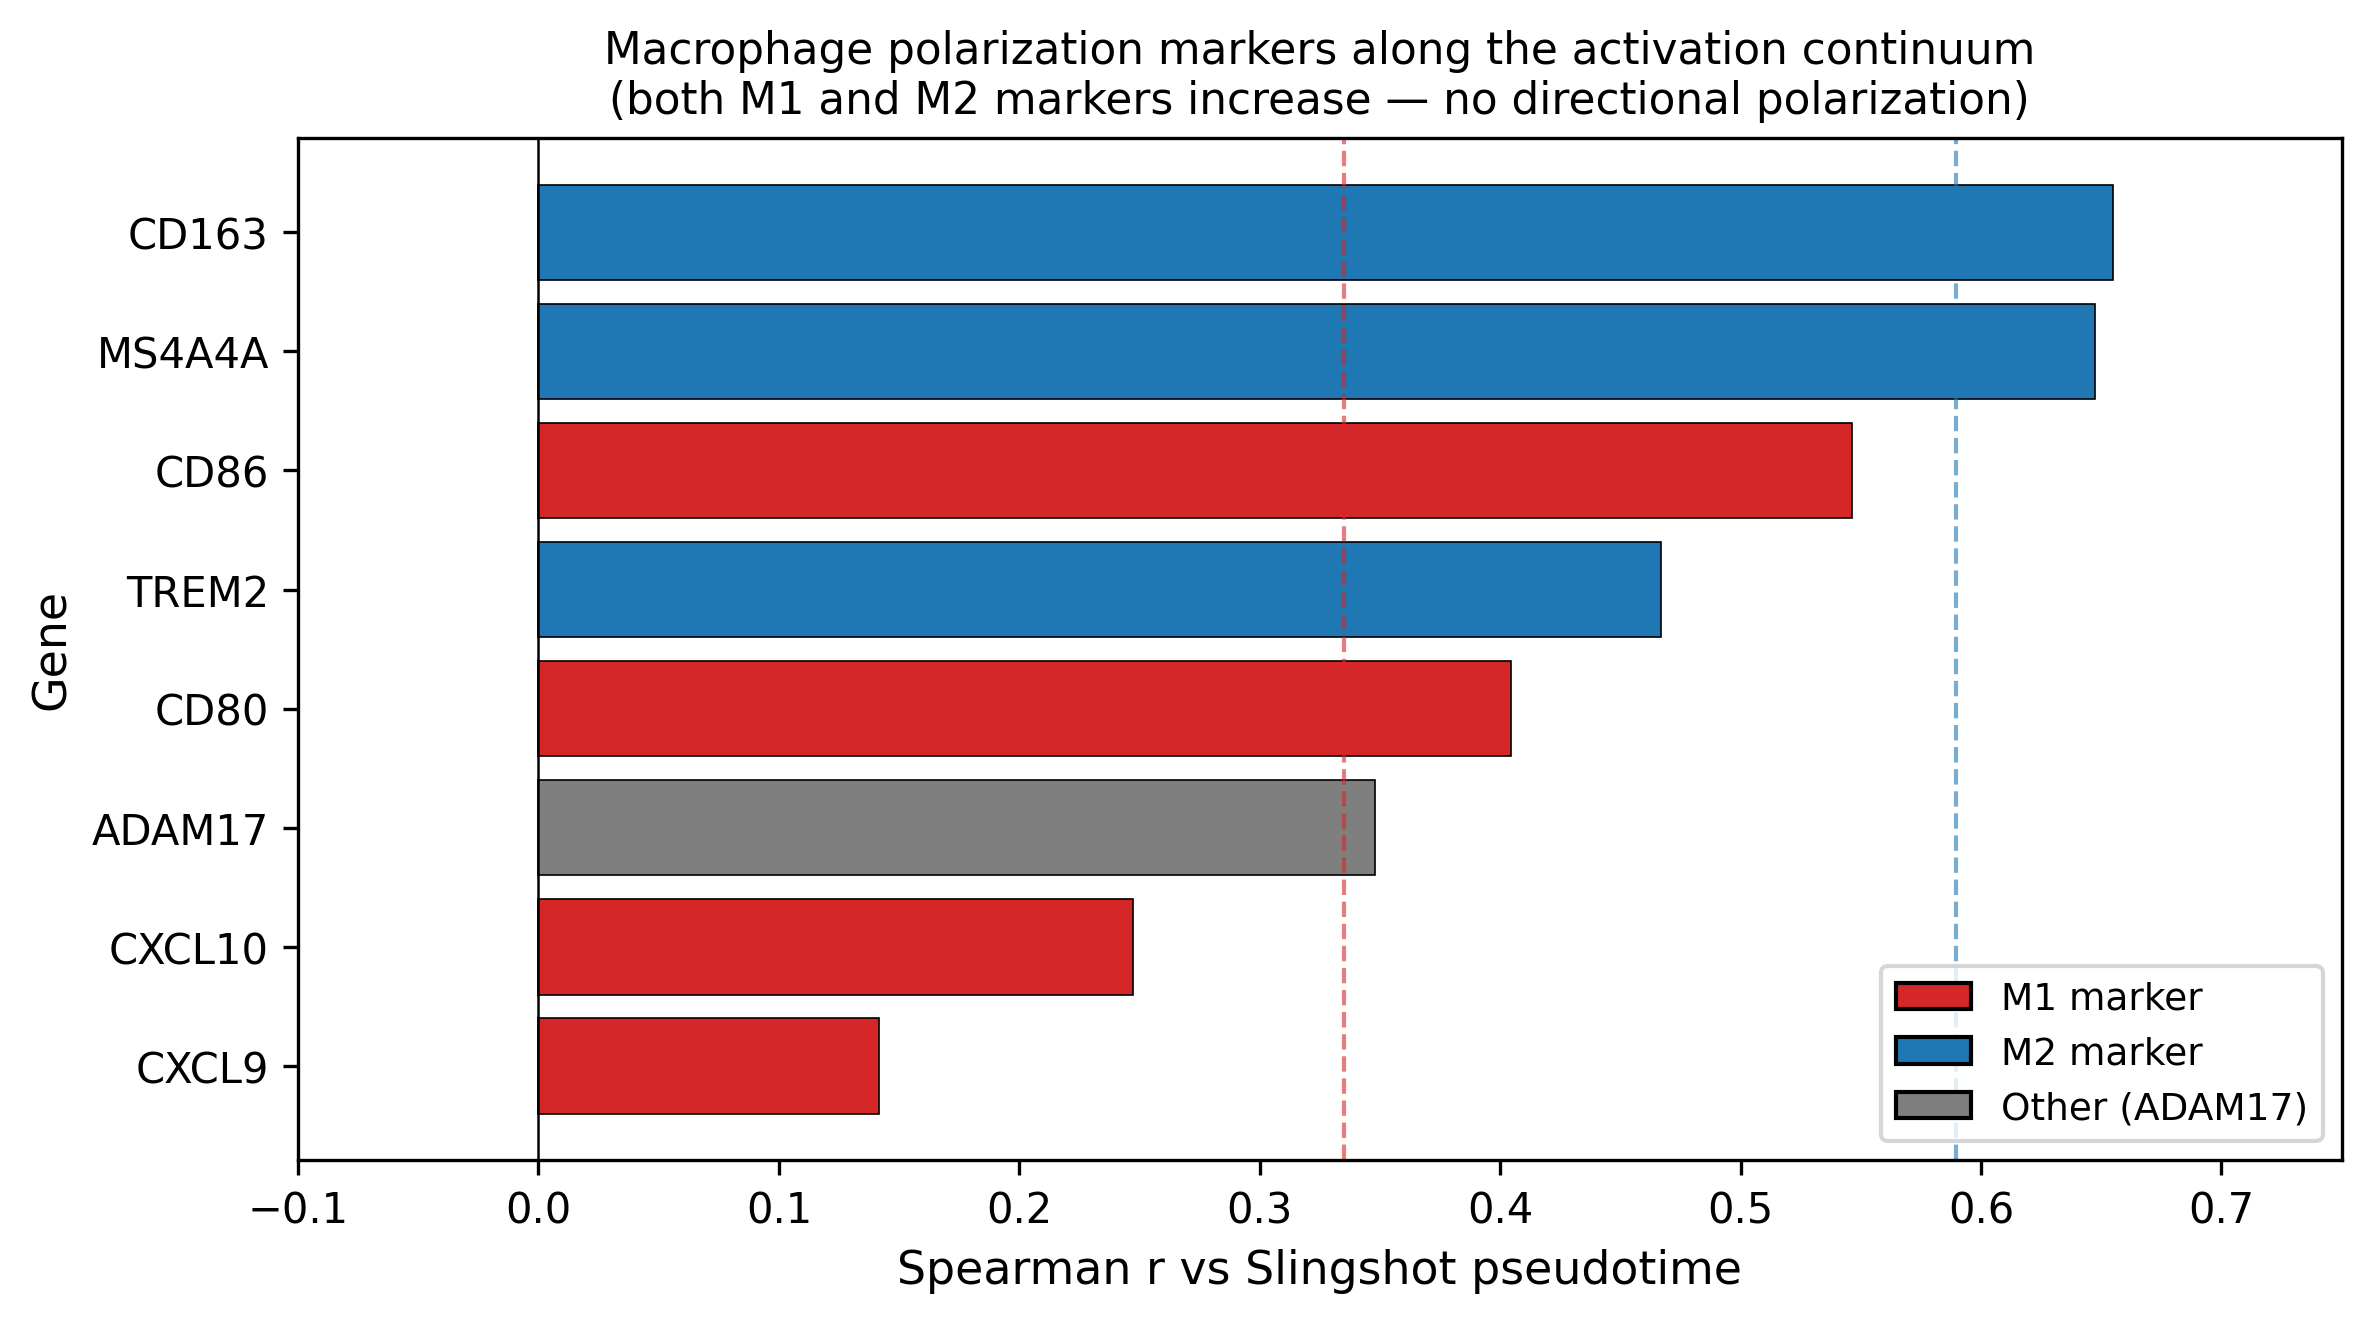
\includegraphics[width=0.85\textwidth]{figures/FigS3_marker_correlations.png}
\caption{\textbf{Los marcadores de polarización correlacionan con pseudotiempo en un patrón no direccional.} Correlación de Spearman $r$ entre el pseudotiempo de Slingshot y la expresión de marcadores canónicos M1 (CD80, CD86, CXCL9, CXCL10) y M2 (CD163, MS4A4A, TREM2), más ADAM17, calculada sobre el compartimento macrofágico de 22{,}902 células. Si el eje de pseudotiempo representara una polarización direccional M1$\to$M2, los marcadores M1 producirían correlaciones negativas y los M2 positivas. En cambio, \emph{ambas} clases muestran correlaciones positivas (M1: media $r = +0.34$, rango $+0.14$ a $+0.55$; M2: media $r = +0.59$, rango $+0.47$ a $+0.65$), con los marcadores M2 aumentando más pronunciadamente. Ésta es la evidencia empírica citada en Resultados~3.5 contra un modelo de polarización direccional y a favor de un continuo de activación global.}
\label{fig:s3}
\end{figure}

\subsection*{Tabla Suplementaria S4 --- Resultados completos de validación Spacia para las 30 interacciones candidatas de LIANA+}
\begin{table}[h!]
\centering
\small
\begin{tabular}{@{}llllrrl@{}}
\toprule
\textbf{Emisor} & \textbf{Receptor} & \textbf{Ligando} & \textbf{Receptor} & \textbf{$\beta$} & \textbf{Spacia $p_{\text{adj}}$} & \textbf{Validado} \\
\midrule
AT1 & Tumor\_resting & ADAM17 & MUC1 & 4.060 & $1.10{\times}10^{-71}$ & \textbf{Sí} \\
Tumor\_resting & AT1 & LTF & AGER & -4.297 & $9.37{\times}10^{-66}$ & \textbf{Sí} \\
Monocyte\_classical & Tumor\_resting & ADAM17 & MUC1 & 2.845 & $8.44{\times}10^{-55}$ & \textbf{Sí} \\
Pericyte & Tumor\_resting & ADAM17 & MUC1 & 1.011 & $3.51{\times}10^{-48}$ & \textbf{Sí} \\
Macrophage\_M1 & Epithelial\_general & ADAM17 & MUC1 & 2.288 & $5.91{\times}10^{-43}$ & \textbf{Sí} \\
Epithelial\_general & Endothelial\_lymphatic & CDH1 & EGFR & 2.184 & $6.64{\times}10^{-42}$ & \textbf{Sí} \\
Epithelial\_general & AT1 & CDH1 & EGFR & 1.939 & $1.18{\times}10^{-32}$ & \textbf{Sí} \\
cDC2 & Tumor\_resting & ADAM17 & MUC1 & 1.839 & $4.97{\times}10^{-31}$ & \textbf{Sí} \\
Macrophage\_M1 & Tumor\_resting & ADAM17 & MUC1 & 1.525 & $4.92{\times}10^{-28}$ & \textbf{Sí} \\
Macrophage\_M2 & Tumor\_resting & ADAM17 & MUC1 & 1.303 & $1.35{\times}10^{-24}$ & \textbf{Sí} \\
cDC1 & AT1 & S100B & AGER & 1.302 & $1.89{\times}10^{-24}$ & \textbf{Sí} \\
Epithelial\_general & Ciliated & CDH1 & EGFR & -0.926 & $6.32{\times}10^{-15}$ & \textbf{Sí} \\
cDC2 & AT1 & S100B & AGER & 0.968 & $4.01{\times}10^{-14}$ & \textbf{Sí} \\
Tumor\_proliferating & AT1 & S100B & AGER & -0.814 & $4.01{\times}10^{-11}$ & \textbf{Sí} \\
pDC & Epithelial\_general & ADAM17 & MUC1 & -0.854 & $1.26{\times}10^{-10}$ & \textbf{Sí} \\
Epithelial\_general & Plasmablast & CDH1 & EGFR & -0.525 & $6.66{\times}10^{-9}$ & \textbf{Sí} \\
Monocyte\_classical & Epithelial\_general & ADAM17 & MUC1 & 0.639 & $1.82{\times}10^{-8}$ & \textbf{Sí} \\
Epithelial\_general & Plasma & CDH1 & EGFR & -0.562 & $2.91{\times}10^{-8}$ & \textbf{Sí} \\
Epithelial\_general & Tumor\_resting & CDH1 & EGFR & -0.005 & $6.27{\times}10^{-7}$ & \textbf{Sí} \\
Ciliated & AT1 & LTF & AGER & -0.233 & $1.17{\times}10^{-4}$ & \textbf{Sí} \\
cDC1 & Tumor\_resting & ADAM17 & MUC1 & 0.172 & 0.048 & Per-test \\
Ciliated & Endothelial\_blood & CD24 & SELP & 0.220 & 0.049 & Per-test \\
pDC & AT1 & S100B & AGER & -0.274 & 0.068 & No \\
Epithelial\_general & Tumor\_resting & ADAM17 & MUC1 & 0.033 & 0.448 & No \\
Pericyte & Epithelial\_general & ADAM17 & MUC1 & -0.430 & 0.545 & No \\
Plasma & Tumor\_resting & ADAM17 & MUC1 & --- & --- & \textit{N/A} \\
pDC & Tumor\_resting & ADAM17 & MUC1 & --- & --- & \textit{N/A} \\
Plasmablast & Tumor\_resting & ADAM17 & MUC1 & --- & --- & \textit{N/A} \\
Plasma & Epithelial\_general & ADAM17 & MUC1 & --- & --- & \textit{N/A} \\
DC\_mature & Tumor\_resting & ADAM17 & MUC1 & --- & --- & \textit{N/A} \\
\bottomrule
\end{tabular}
\caption{\textbf{Tabla completa de validación Spacia para las 30 interacciones candidatas de LIANA+.} Columnas: tipos celulares emisor y receptor; ligando y receptor (primer gen listado para complejos multi-subunidad, ver Métodos); coeficiente $\beta$ a nivel de vía (el signo indica la dirección de enriquecimiento espacial); $p$-value ajustado de Spacia a nivel de vía; resultado de validación dual bajo corrección de Bonferroni sobre las 30 pruebas cruzadas ($p_{\text{adj}} < 1.67 \times 10^{-3}$). Cinco filas tienen celdas $\beta$/$p$-value vacías: corresponden a ajustes Spacia que no completaron porque el tipo celular emisor contenía menos de 500 células (Plasma, Plasmablast, DC madura, y pDC); se reportan transparentemente como inconclusas en lugar de excluirlas a priori. Fuente por fila: \texttt{human\_lung\_cancer/results/02\_biology/phase\_f\_spacia/F3\_spacia\_results.csv}.}
\label{tab:s4}
\end{table}

\end{document}
